\documentclass[titlepage]{jsarticle}
\usepackage[dvipdfmx]{graphicx}
\usepackage{amsmath}
\usepackage{amssymb}
\usepackage{amsfonts}
\usepackage{comment}
\usepackage{h31ec-exp}
\usepackage{listings}
\lstset{
    basicstyle={\ttfamily},
    identifierstyle={\small},
    commentstyle={\smallitshape},
    keywordstyle={\small\bfseries},
    ndkeywordstyle={\small},
    stringstyle={\small\ttfamily},
    frame={tb},
    breaklines=true,
    columns=[l]{fullflexible},
    numbers=left,
    xrightmargin=0zw,
    xleftmargin=3zw,
    numberstyle={\scriptsize},
    stepnumber=1,
    numbersep=1zw,
    lineskip=-0.5ex,
    keepspaces=true,
    language=c
}
\renewcommand{\lstlistingname}{リスト}
\makeatletter
\newcommand{\figcaption}[1]{\def\@captype{figure}\caption{#1}}
\newcommand{\tblcaption}[1]{\def\@captype{table}\caption{#1}}
\makeatother

\title{数値シミュレーション}
\grade{4年32番}
\author{平田 蓮}
\team{}
\date{2020年11月6日}
\expdate{2020年10月15日, 10月22日, 10月29日, 11月5日}
\coauthor{}

\begin{document}
\maketitle
\section{目的}
    この実験では, 実際の系をモデルに置き換えてシミュレーションすることで挙動を調べる.
    しかし, シミュレーションがうまくいくとは限らないので,
    シミュレーションの結果を鵜呑みにせず,
    その結果の妥当性を検証して確かめることが大切である.

    この実験を通して, 様々な方向からのシミュレーション結果の解析方法を身に付けることを目的とする.

\section{バネ-マス-ダンパ系のシミュレーション}
    この節では, 実験テキスト\cite{text}のFig.25に示されているバネ-マス-ダンパ系のシミュレーションを行う.
    \subsection{系の運動方程式}
        まずはシミュレーションモデルを構成するために系の運動方程式を導出する.

        図より, 運動方程式は次のようになる.

        \[
            m \ddot{x}(t) = f(t) -kx(t) - c \dot{x}(t)
        \]

        次小節でモデルを構築するために左辺を$\ddot{x}(t)$の形にすると,

        \begin{equation}
            \ddot{x}(t) = \frac{f_0}{m} u(t) -\frac{k}{m}x(t) - \frac{c}{m} \dot{x}(t) \label{equ:fma}
        \end{equation}

        となる.

    \subsection{シミュレーションモデルの構築}
        式(\ref{equ:fma})に基づいて構築したモデルを図\ref{fig:bmdsim}に示す.

        \begin{figure}[h]
            \centering
            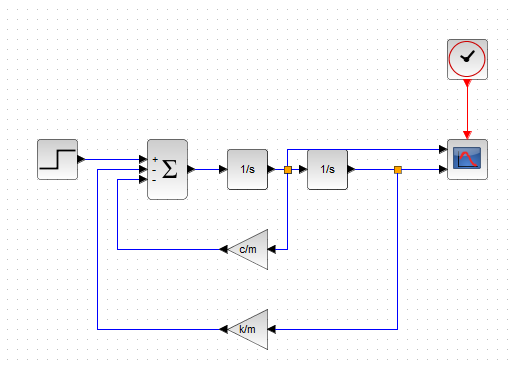
\includegraphics[width=10cm]{img/BMDsim.png}
            \caption{バネ-マス-ダンパ系のシミュレーションモデル}
            \label{fig:bmdsim}
        \end{figure}

        総和ブロックの出力を$\ddot{x}(t)$と考え,
        $\displaystyle \frac{1}{s}$のブロック二つを通して$x(t)$まで積分処理を施している.
        よって, 一回だけ積分をした点は$\dot{x}(t)$である.

        運動方程式に基づき, $\dot{x} (t), x(t)$それぞれに
        $\displaystyle \frac{c}{m}, \frac{k}{m}$を掛けて負帰還をしている.

        また, 物体に加わり続ける外力として, 大きさ$f_0$のステップ入力を総和ブロックに加えている.

        最後に, $x(t)$と$\dot{x}(t)$を出力として得たいので, それらを出力ブロックに入力している.

    \subsection{パラメータの計算} \label{sec:para}
        シミュレーションをする際の定数として各値を計算する.
        各値は次のように与えられている.

        \begin{eqnarray*}
            m &=& 出席番号\times 100 \ \mathrm{kg} \\
            k &=& \frac{|150 + (出席番号-25)^2\times 50|}{10} \ \mathrm{kg/s^2} \\
            c &=& 650-(出席番号-25)^2 \ \mathrm{kg/s} \\
            f_0 &=& 300 \ \mathrm{kg \cdot cm/s^2}
        \end{eqnarray*}

        私の出席番号は32であるので,
        これを代入して各値を計算すると,

        \begin{eqnarray*}
            m &=& 32 \times 100 = 3200 \ \mathrm{kg} \\
            k &=& \frac{|150 + (32-25)^2\times 50|}{10} = 260 \ \mathrm{kg/s^2} \\
            c &=& 650-(32-25)^2 = 601 \ \mathrm{kg/s}
        \end{eqnarray*}

        を得られる.

        これらを式(\ref{equ:fma})に代入すると,

        \[
            \ddot{x}(t) \approx 0.09375 u(t) -0.08125x(t) -0.18781 \dot{x}(t)
        \]

        となる.
        
    \subsection{シミュレーション結果}
        構築したモデルと求めたパラメータを使いシミュレーションを行った結果を図\ref{fig:bmd}に示す.

        \begin{figure}[h]
            \centering
            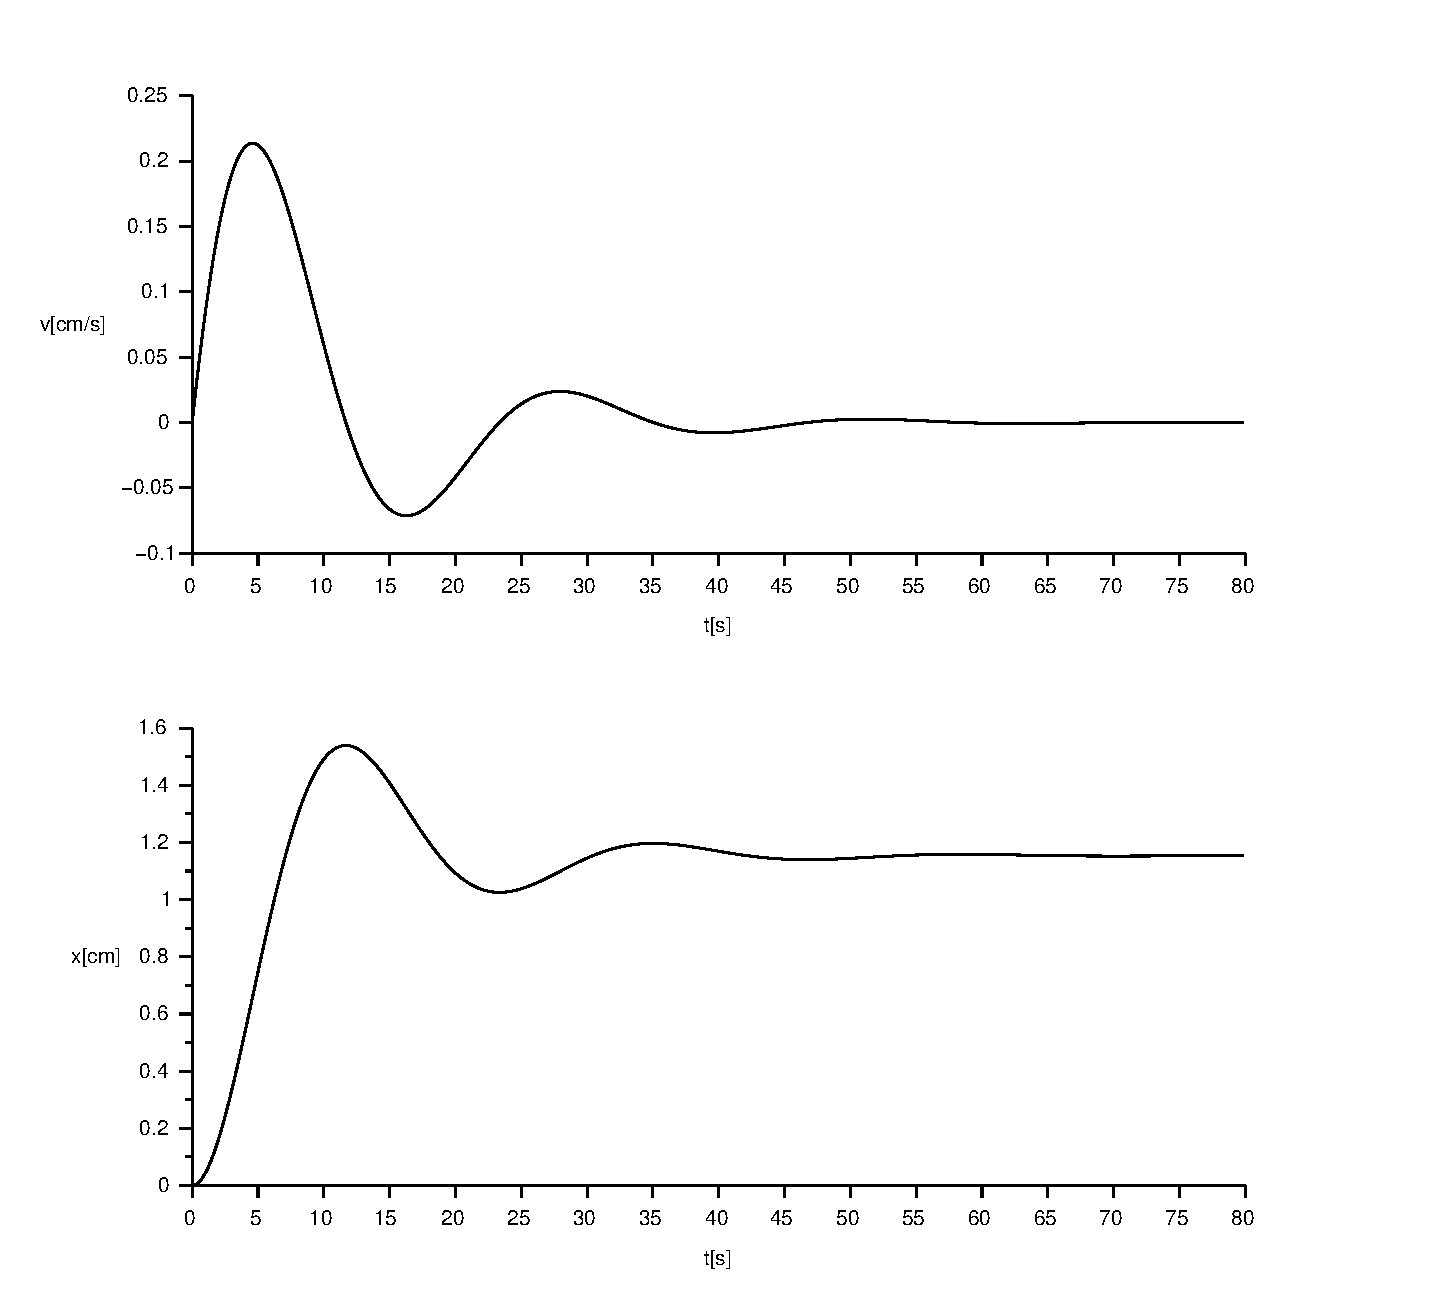
\includegraphics[width=15cm]{img/BMD.eps}
            \caption{バネ-マス-ダンパ系のシミュレーション結果}
            \label{fig:bmd}
        \end{figure}

        上のグラフは$v(t) (=\dot{x}(t))$, 下のグラフは$x(t)$を示している.
        
    \subsection{結果の解析}
        前小節で行ったシミュレーションの結果の妥当性を調べるために解析を行う.

        \subsubsection{pythonを使ったシミュレーション}
            まずはじめに, 本質的には同じことであるが,
            Scilabではない別のソフトウェアを使ってシミュレーションを行ってみる.
            今回はプログラミング言語Pythonを使ってシミュレーションする.

            作成したコードをリスト\ref{lst:bmdpy}に示す.

            \begin{lstlisting}[caption=simulate.py, label=lst:bmdpy]
import numpy as np
from scipy.integrate import odeint
import matplotlib.pyplot as plt

def f(x, t):
    return (x[1], 0.09375 - 0.08125 * x[0] - 0.18781 * x[1])

x0 = [0, 0]
t = np.linspace(0, 80, 1000)
y = odeint(f, x0, t)

fig = plt.figure()
s1 = fig.add_subplot(2, 1, 1)
s2 = fig.add_subplot(2, 1, 2)

s2.plot(
    t, y[:,[0]],
    color='k'
)
s2.set_xlabel('t[s]')
s2.set_xlim([0, 80])
s2.set_ylabel('x[cm]', rotation=0)
s2.set_ylim([0, 1.6])

s1.plot(
    t, y[:,[1]],
    color='k'
)
s1.set_xlabel('t[s]')
s1.set_xlim([0, 80])
s1.set_ylabel('v[cm/s]', rotation=0)
s1.set_ylim([-0.1, 0.25])

plt.show()\end{lstlisting}

            scipyというライブラリの\verb|integrate.odeint()|という関数を使用して
            値をシミュレーションをする.

            シミュレーション結果を図\ref{fig:bmdpy}に示す.

            \begin{figure}[h]
                \centering
                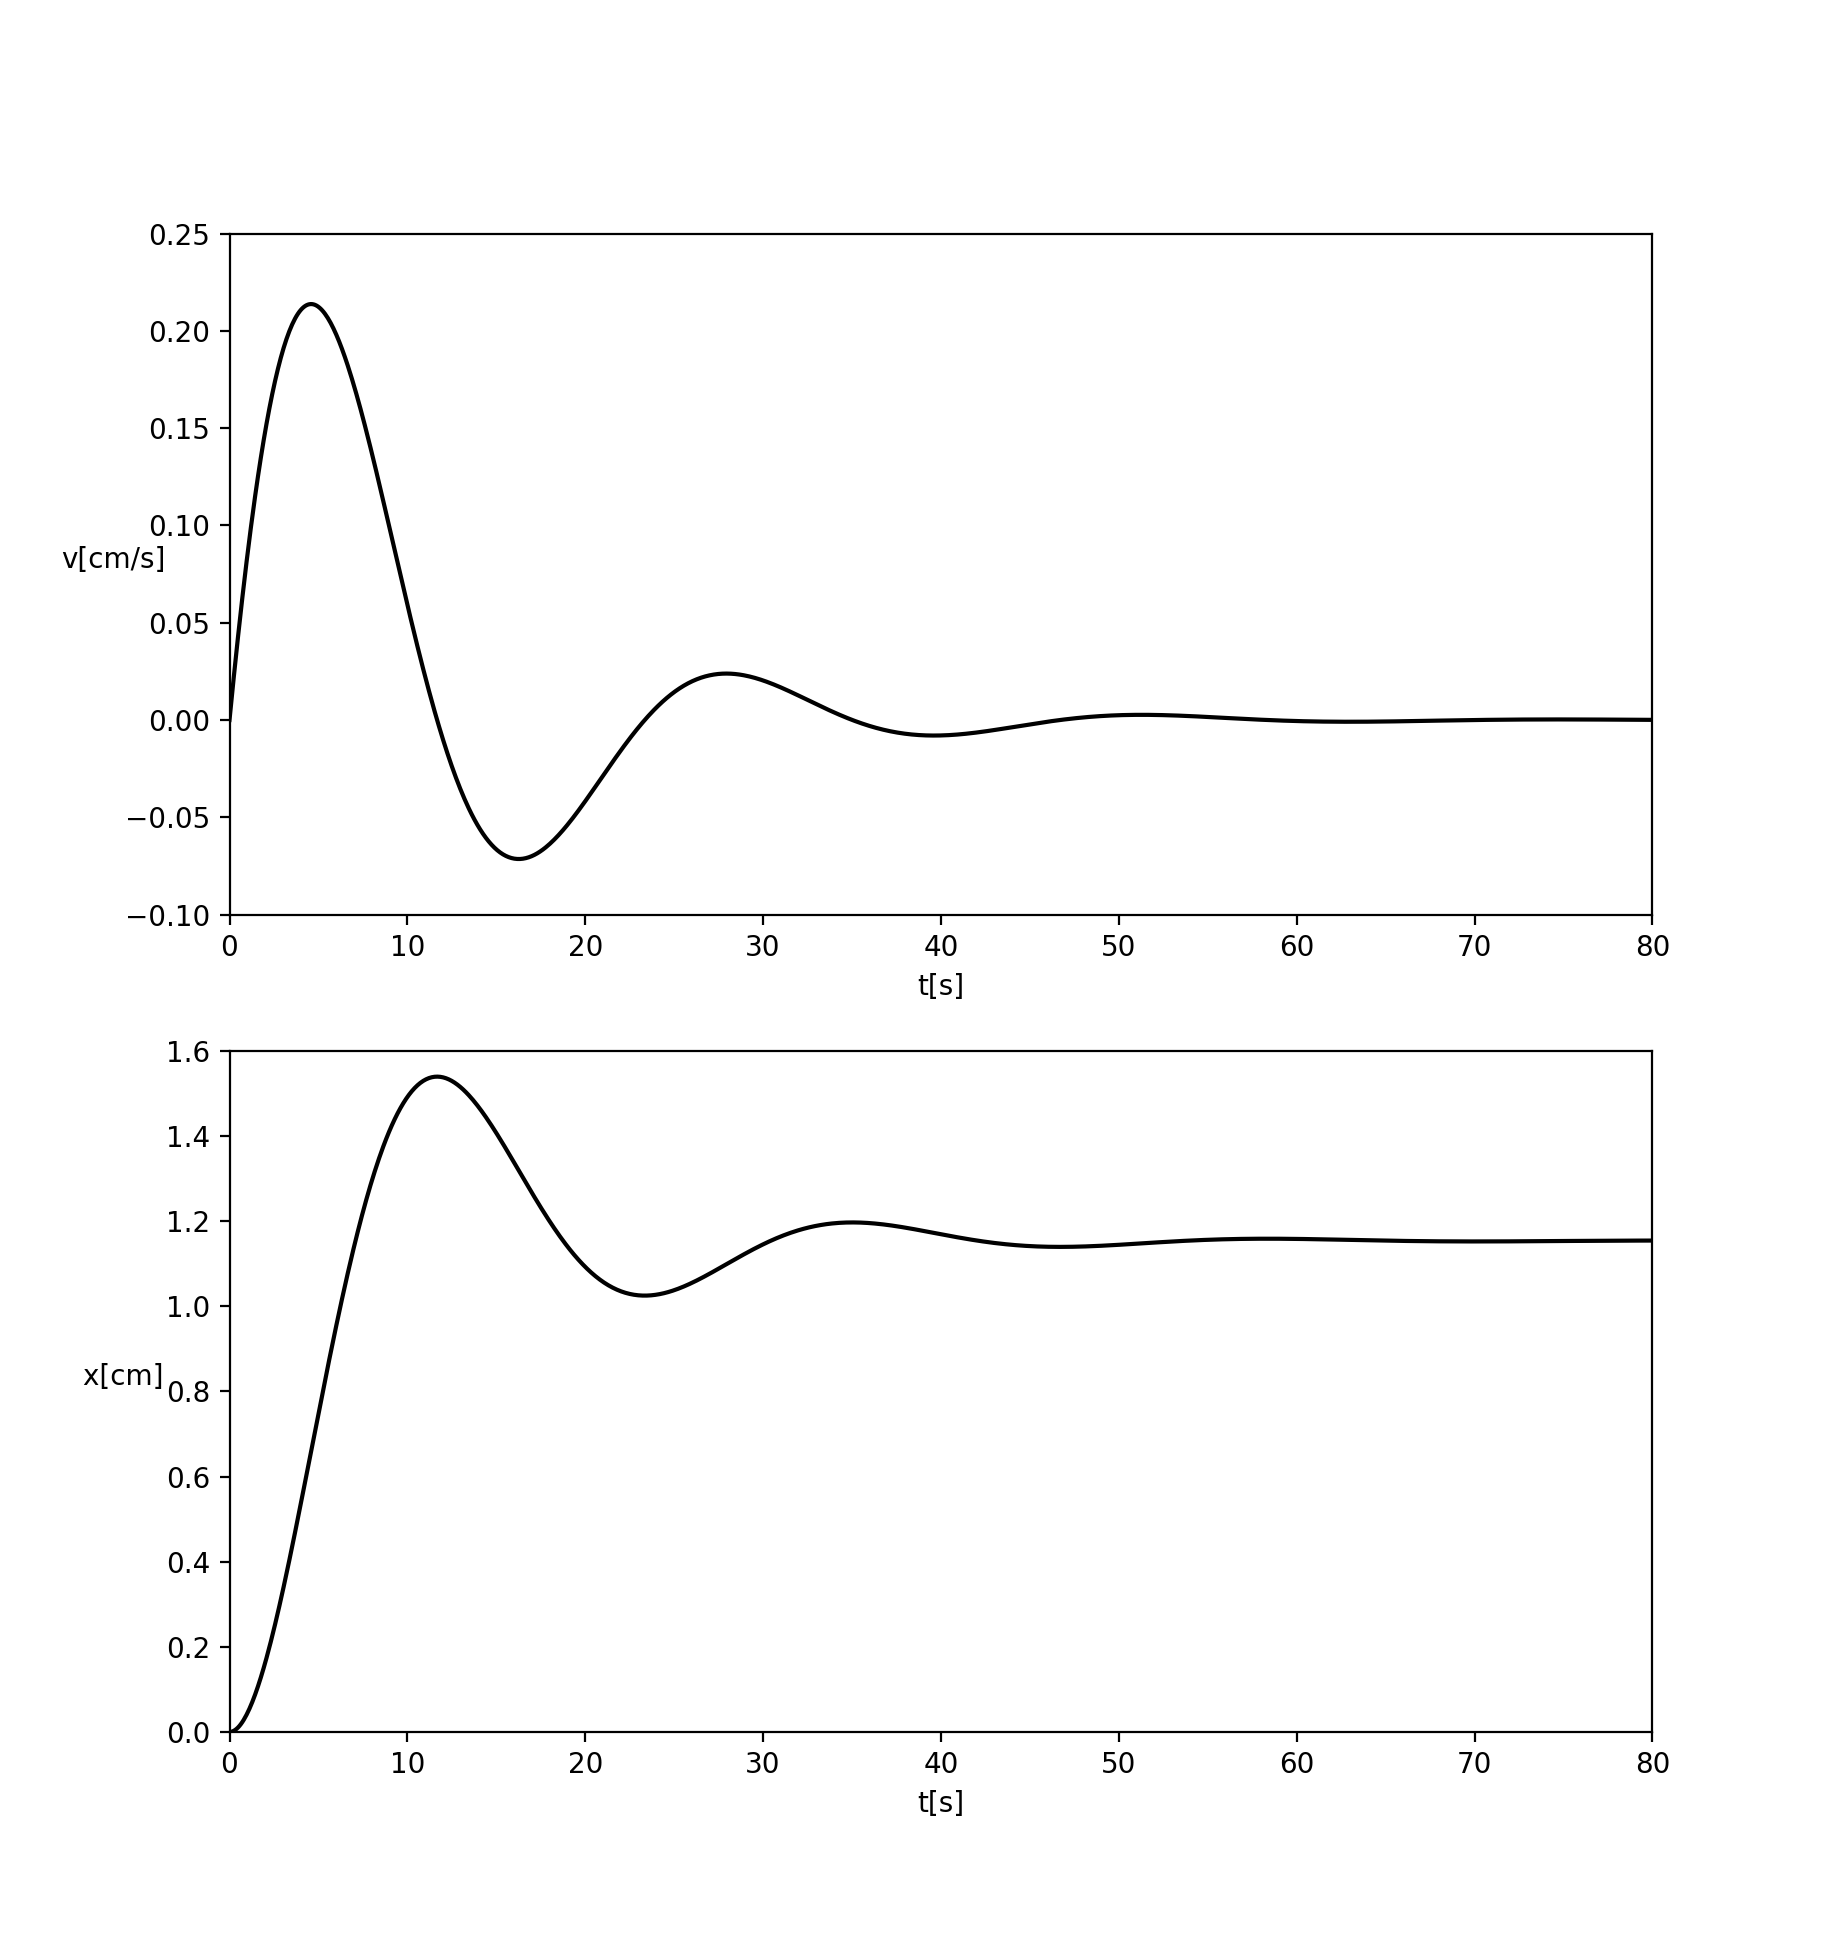
\includegraphics[width=15cm]{img/bmdpy.png}
                \caption{バネ-マス-ダンパ系のPythonによるシミュレーション結果}
                \label{fig:bmdpy}
            \end{figure}

            図\ref{fig:bmd}と比べてみても, 同様の結果が出ていることがわかる.
            
        \subsubsection{初期値, 最終値の定理}
            $\mathcal{L}[f(t)] = F(s)$として初期値の定理, 最終値の定理を式(\ref{equ:lim0}), (\ref{equ:liminf})に示す.

            \begin{eqnarray}
                \lim_{s \to \infty} sF(s) &=& \lim_{t \to +0} f(t) \label{equ:lim0} \\
                \lim_{s \to 0} sF(s) &=& \lim_{t \to \infty} f(t) \label{equ:liminf}
            \end{eqnarray}

            これらを使うために式(\ref{equ:fma})の両辺をラプラス変換する.
            初期条件を$x(0) = v(0) = 0$とすると,

            \begin{eqnarray*}
                s^2 X(s) &=& \frac{f_0}{m} \frac{1}{s} - \frac{k}{m} X(s) - \frac{c}{m} sX(s) \\
                \leftrightarrow X(s) &=& \frac{f_0}{s(ms^2+cs+k)}
            \end{eqnarray*}

            \ref{sec:para}で計算したパラメータを代入して,
            
            \begin{equation}
                X(s) = \frac{300}{s(3200s^2+601s+260)} \label{equ:lap}
            \end{equation}

            となる.

            まず初期値の定理より,

            \[
                \lim_{t \to +0} x(t) = \lim_{s \to \infty} sX(s) = \lim_{s \to \infty} \frac{300}{3200s^2+601s+260} = 0
            \]

            次に最終値の定理より,

            \[
                \lim_{t \to \infty} x(t) = \lim_{s \to 0} sX(s) = \lim_{s \to 0} \frac{300}{3200s^2+601s+260} \approx 1.154
            \]

            また, $\mathcal{L}[v(t)] = sX(s)$であるので,

            \begin{eqnarray*}
                \lim_{t \to +0} v(t) &=& \lim_{s \to \infty} s^2X(s) = \lim_{s \to \infty} \frac{300}{3200s+601+260s^{-1}} = 0 \\
                \lim_{t \to \infty} v(t) &=& \lim_{s \to 0} s^2X(s) = \lim_{s \to 0} \frac{300}{3200s+601+260s^{-1}} = 0
            \end{eqnarray*}

            となる.
            図\ref{fig:bmd}, \ref{fig:bmdpy}をみると, これらの値がみて取れるため,
            少なくとも初期値と最終値のシミュレーションは正しいことがわかる.
            
        \subsubsection{運動方程式の解}
            次に, 運動方程式の解を求めることで$x(t), v(t)$を直接グラフ化してみる.

            まず, 式(\ref{equ:lap})の両辺を逆ラプラス変換して$x(t)$を求める.

            \begin{eqnarray}
                x(t) &=& \mathcal{L}^{-1}\left[\frac{300}{s(3200s^2+601s+260)}\right] \nonumber \\
                &\approx& 1.154\mathcal{L}^{-1}\left[\frac{1}{s} - \frac{s+0.0939}{(s+0.0939)^2 + 0.2691^2}\right] \nonumber \\
                &=& 1.154(1 - e^{-0.0939t}\cos{0.2691t}) \label{equ:x}
            \end{eqnarray}

            次に, $sX(s)$をラプラス逆変換して$v(t)$を得る.

            \begin{eqnarray}
                v(t) &=& \mathcal{L}^{-1}\left[\frac{300}{3200s^2 + 601s + 260}\right] \nonumber \\
                &\approx& 0.3483 e^{-0.0939t}\sin{0.2691t} \label{equ:v}
            \end{eqnarray}

            式(\ref{equ:x}), (\ref{equ:v})をグラフ化したものを図\ref{fig:bmdplot}に示す.

            \begin{figure}[h]
                \centering
                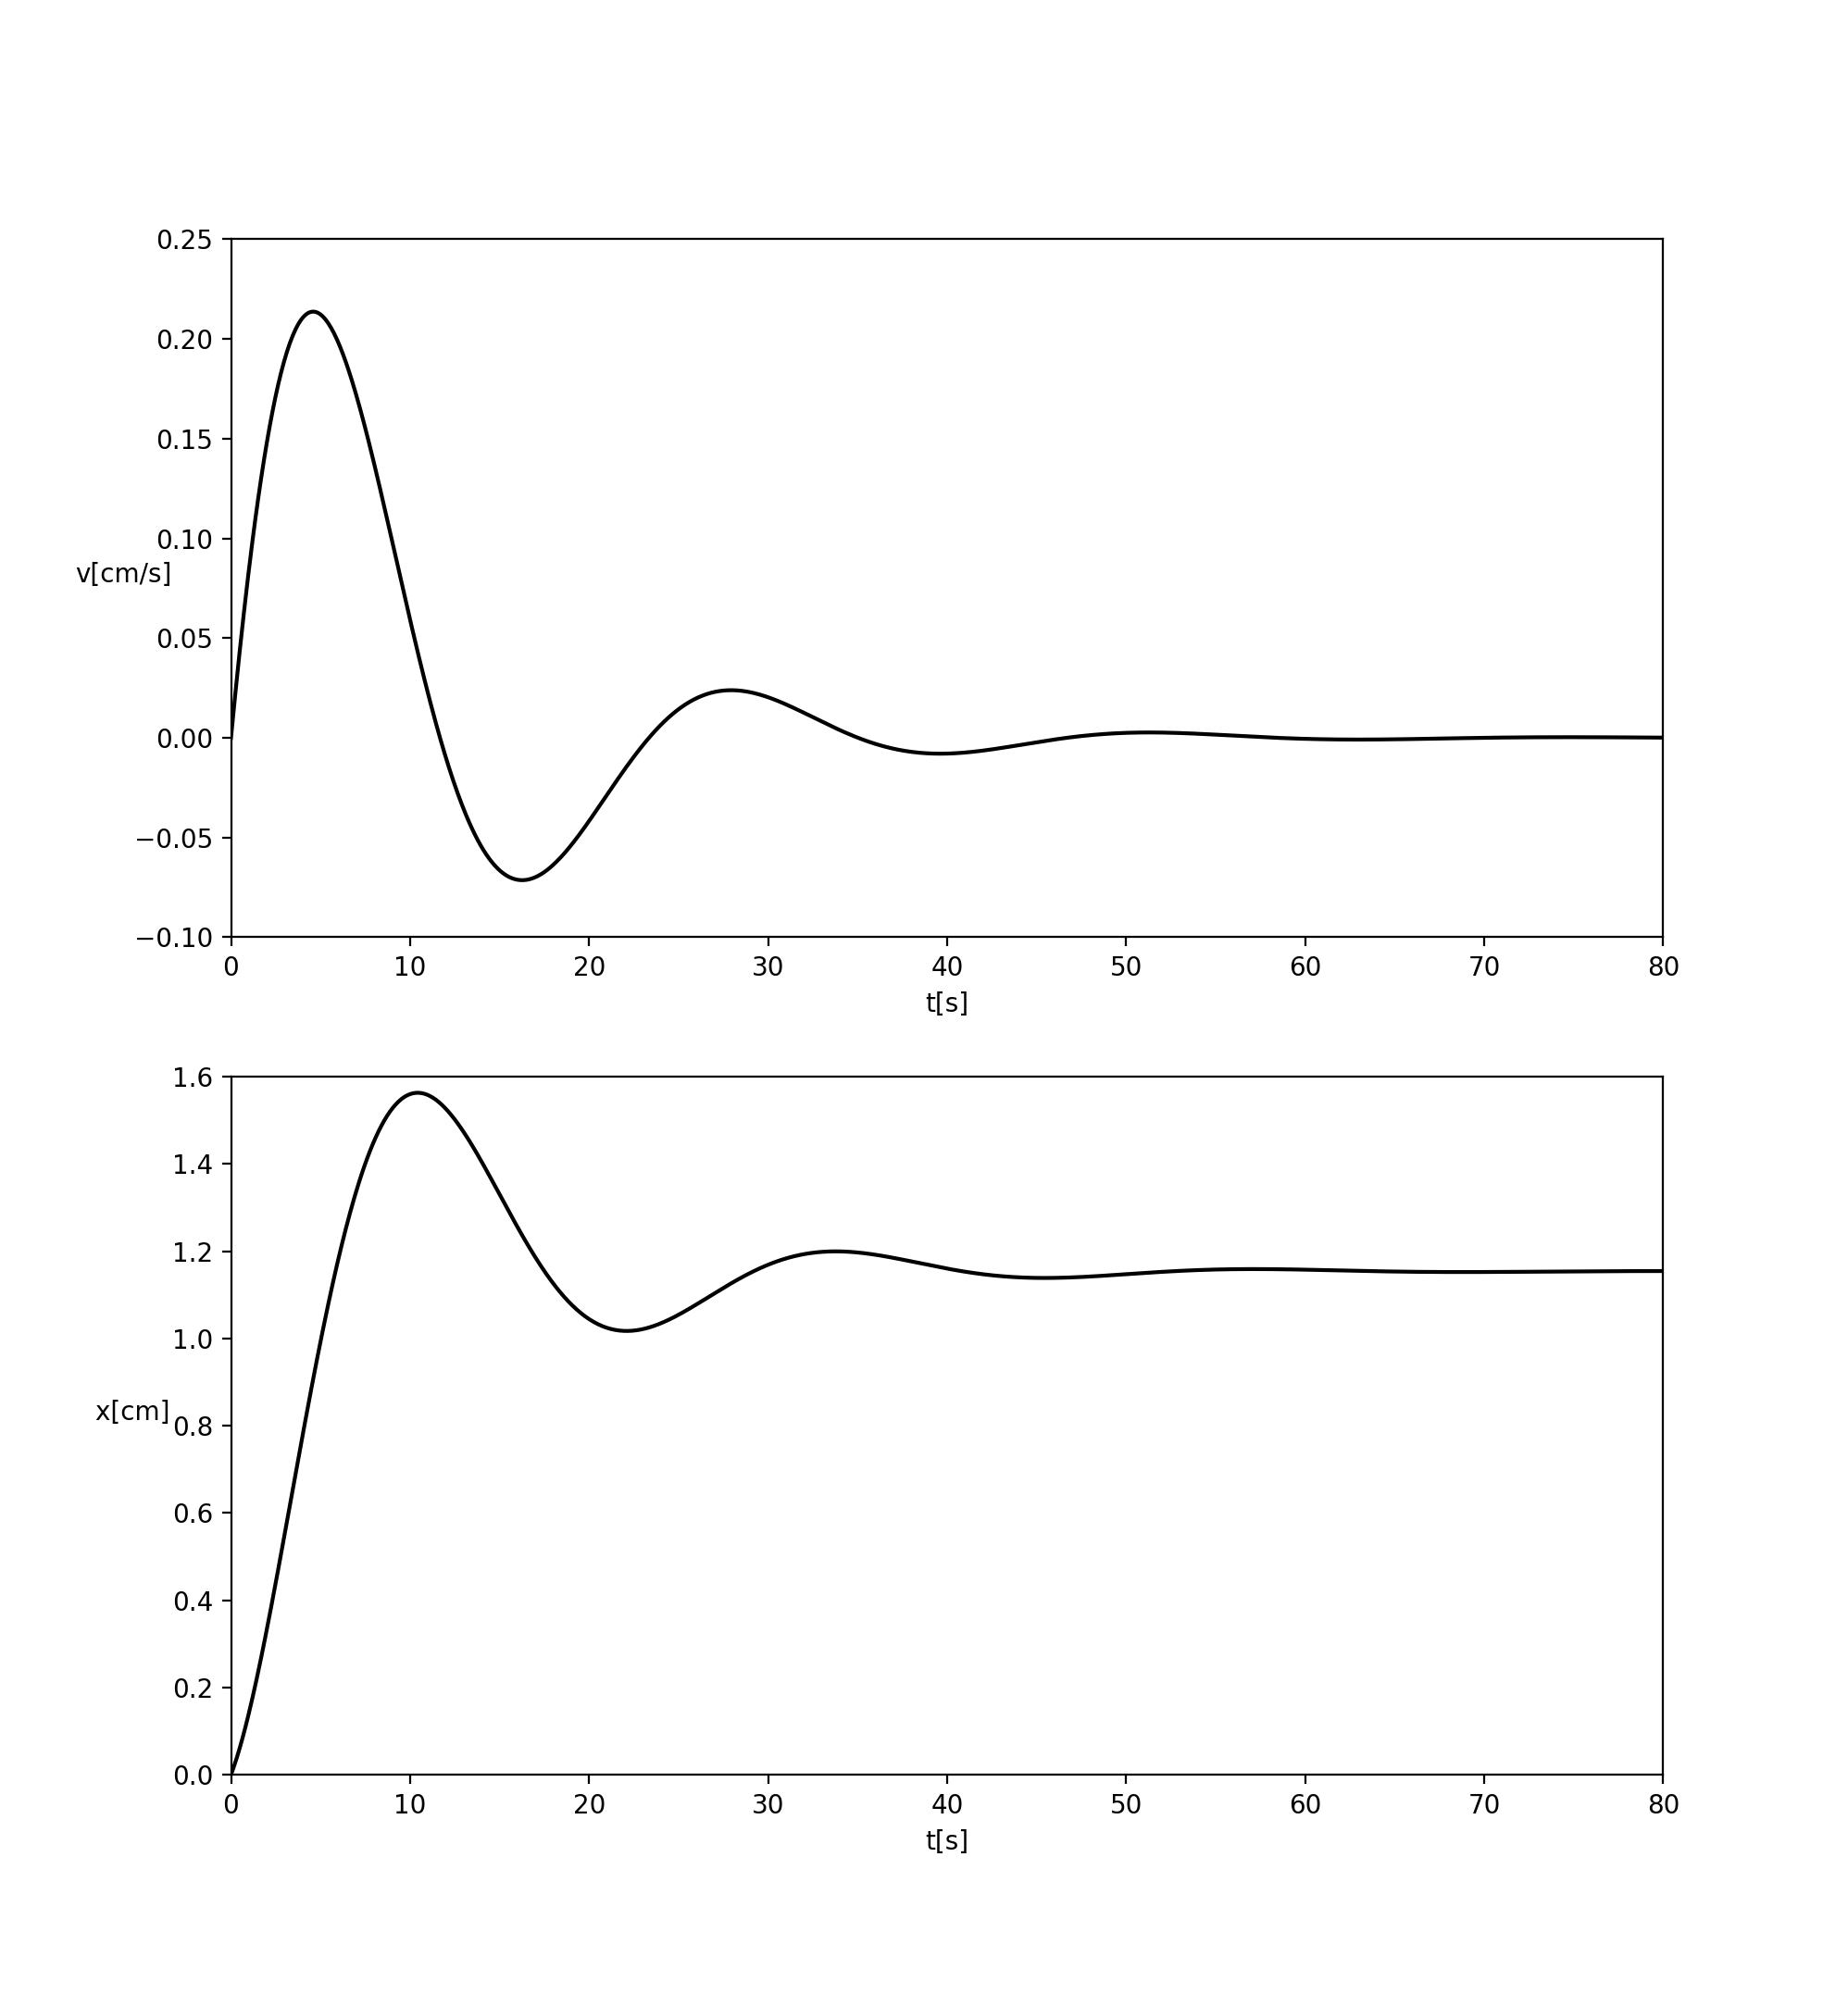
\includegraphics[width=15cm]{img/bmdplt.png}
                \caption{$x(t), v(t)$のプロット}
                \label{fig:bmdplot}
            \end{figure}

            グラフより, シミュレーションが正確であったと言える.

            ここで, $v(t) = \dot{x}(t)$であることに着目すると,
            $sX(s)$をラプラス変換するのではなく, \ $x(t)$を$t$で微分することで
            $v(t)$を得られるのではないかと考えることができる.
            そのように求める$v(t)$を$v_f(t)$とすると, 式(\ref{equ:fakev})のようになる.

            \begin{eqnarray}
                v_f(t) &\approx& 1.154 e^{-0.0939 t} (0.2691 \sin{0.2691 t} + 0.0939 \cos{0.2691 t}) \nonumber \\
                &\approx& e^{-0.0939 t} (0.3105\sin{0.2691t} + 0.1084 \cos{0.2691t}) \label{equ:fakev}
            \end{eqnarray}

            これを式(\ref{equ:v})とプロットして比較してみると,
            図\ref{fig:versus}のようになる.

            \begin{figure}[h]
                \centering
                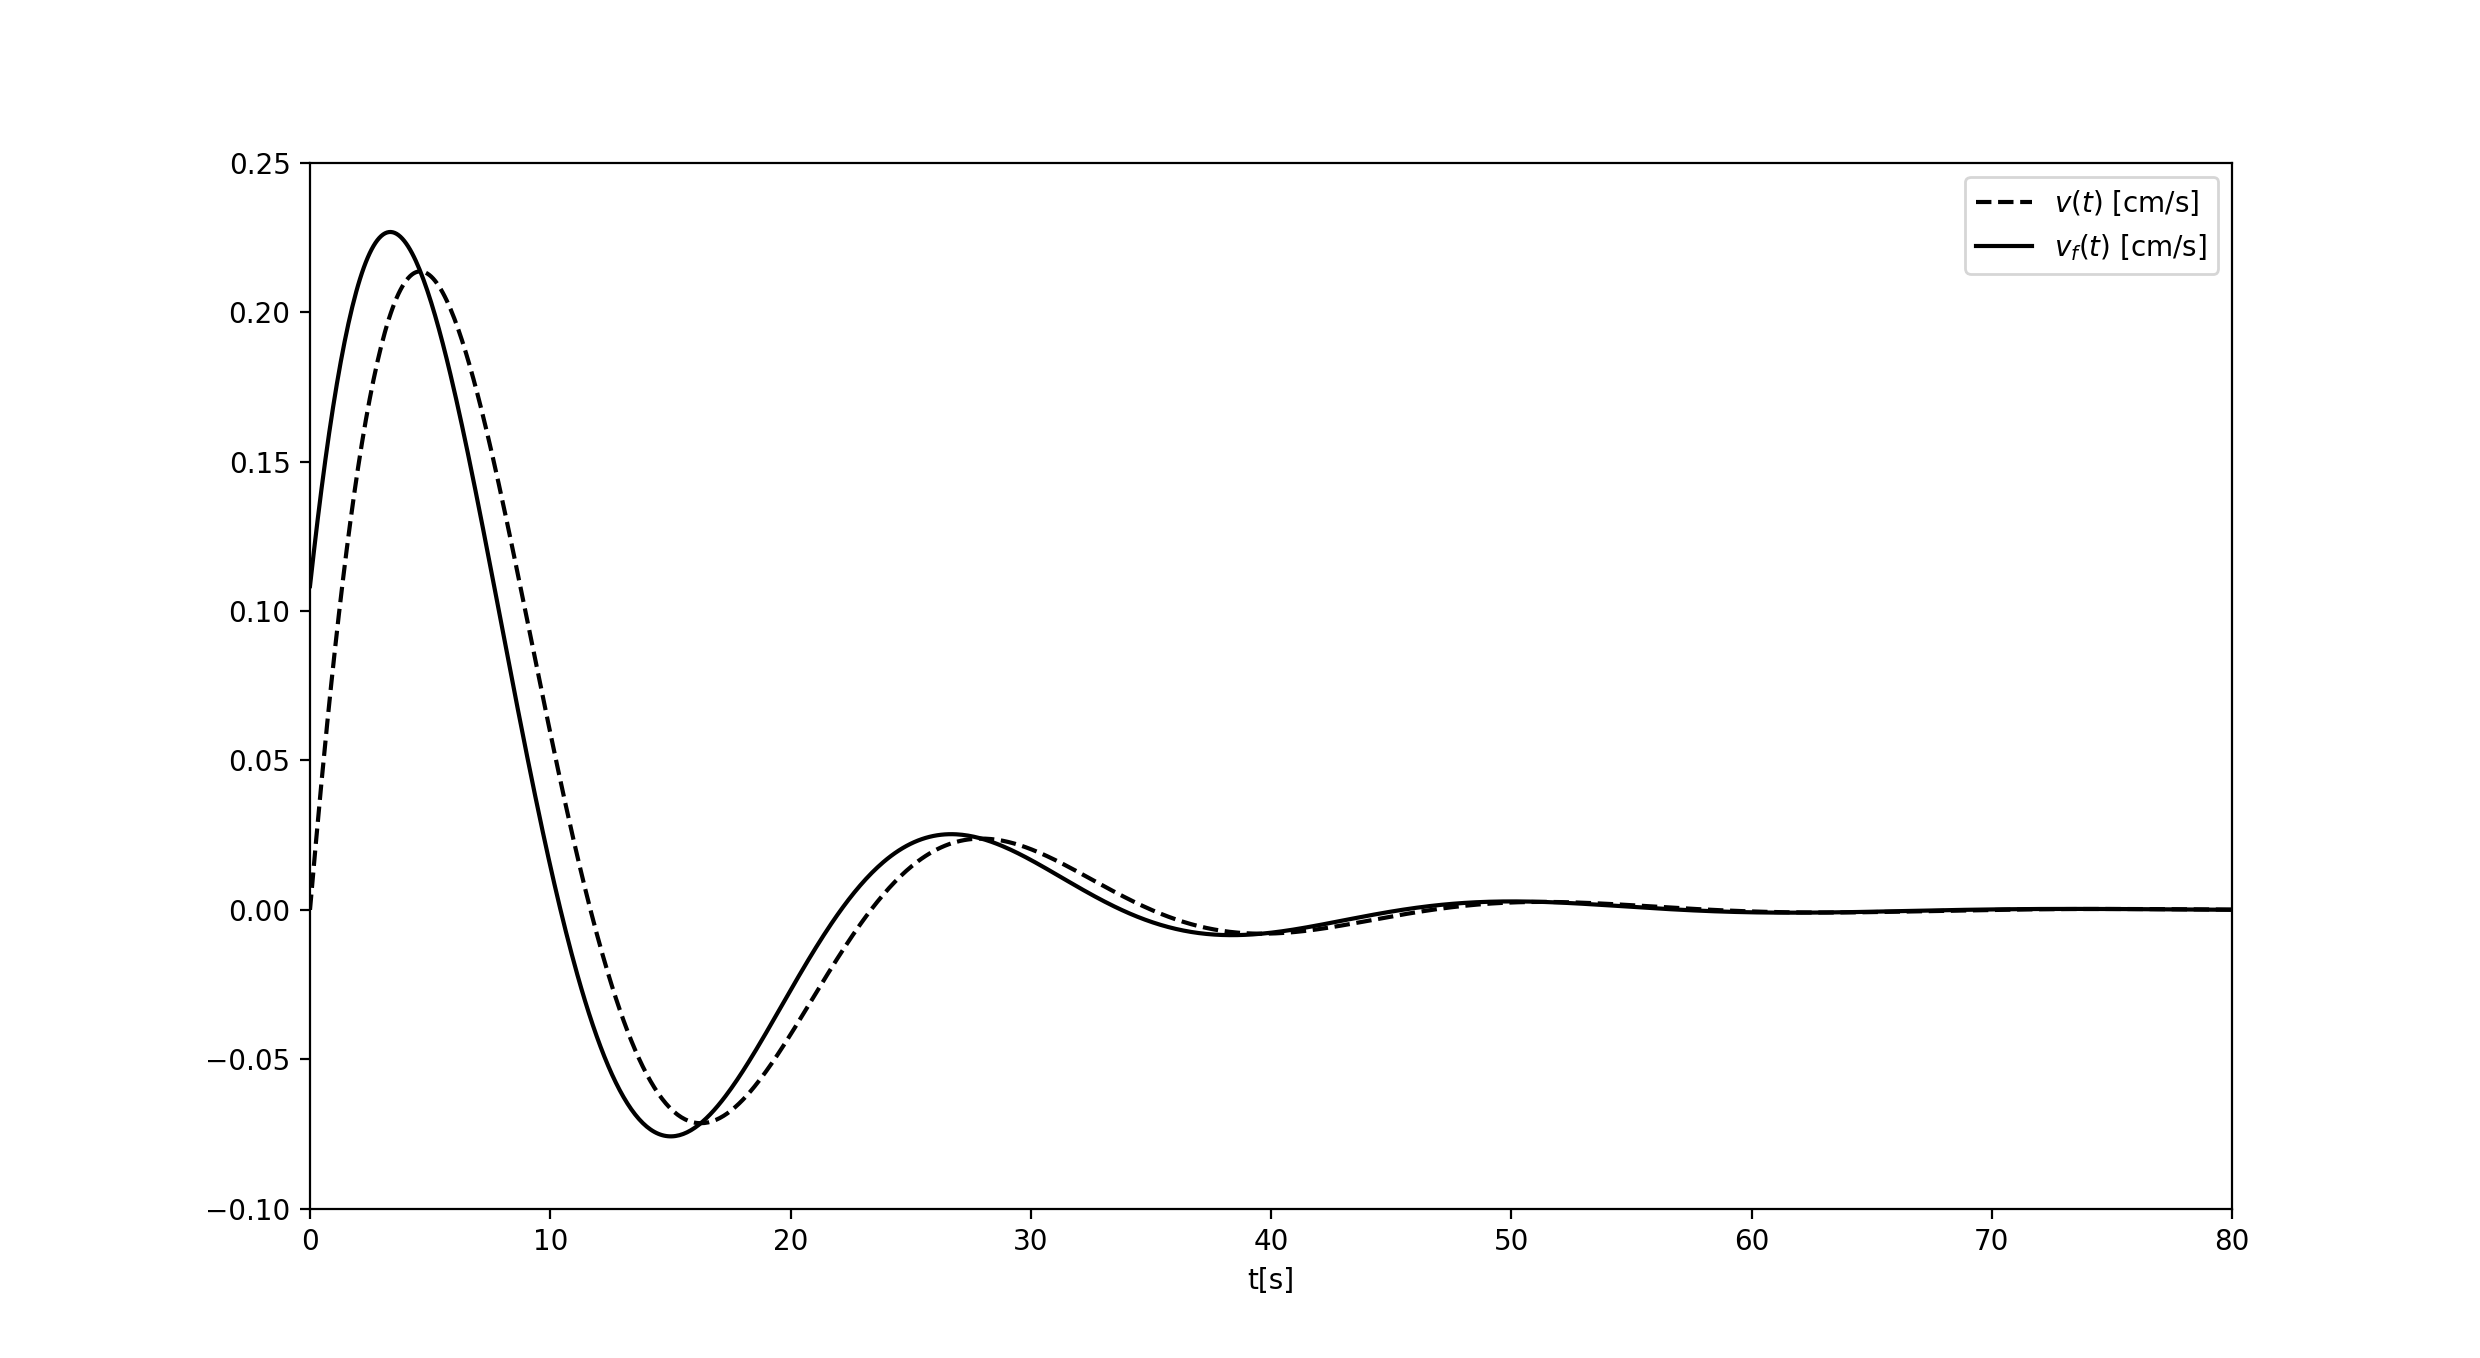
\includegraphics[width=15cm]{img/versus.png}
                \caption{$v(t), v_f(t)$のプロット}
                \label{fig:versus}
            \end{figure}

            グラフより, $v_f(t)$は$v(t)$の振幅を少しだけ大きくし,
            位相を少しだけ早めたものであると考えられる.

            この差は初期条件$v(0) = 0$を考慮しているか,
            また, $t < 0$の領域を考慮しているかどうかによって現れている
            と考えられる.
            実際に, $v_f(t)が0$となる$t$では$x(t)$が
            極値を迎えているが,
            $v(t) = 0$となる点はずれている.

            これは以下の計算によって確かめられる.

            \begin{eqnarray*}
                v(t) &\approx& 0.3483 e^{-0.0939t}\sin{0.2691t} = 0 \\
                \leftrightarrow \sin{0.2691t} &=& 0 \\
                \leftrightarrow 0.2691t &=& n \pi \ (n \in \mathbb{Z}) \\
                \leftrightarrow t &\approx& 11.674n \\ \\
                v_f(t) &\approx& e^{-0.0939 t} (0.3105\sin{0.2691t} + 0.1084 \cos{0.2691t}) = 0 \\
                \leftrightarrow \tan{0.2691t} &=& -0.3491 \\
                \leftrightarrow t &\approx& n \pi - 1.2481 \ (n \in \mathbb{Z}) \\
                \leftrightarrow t &\approx& 11.674n - 1.2481
            \end{eqnarray*}

            $n = 1$の点について,
            $v(t) \approx 0 \leftrightarrow t = 11.674$,
            $v_f(t) \approx 0 \leftrightarrow t = 10.426$である.

            この範囲に絞って$x(t)$をプロットしてみると,
            図\ref{fig:surp}となる.

            \begin{figure}[h]
                \centering
                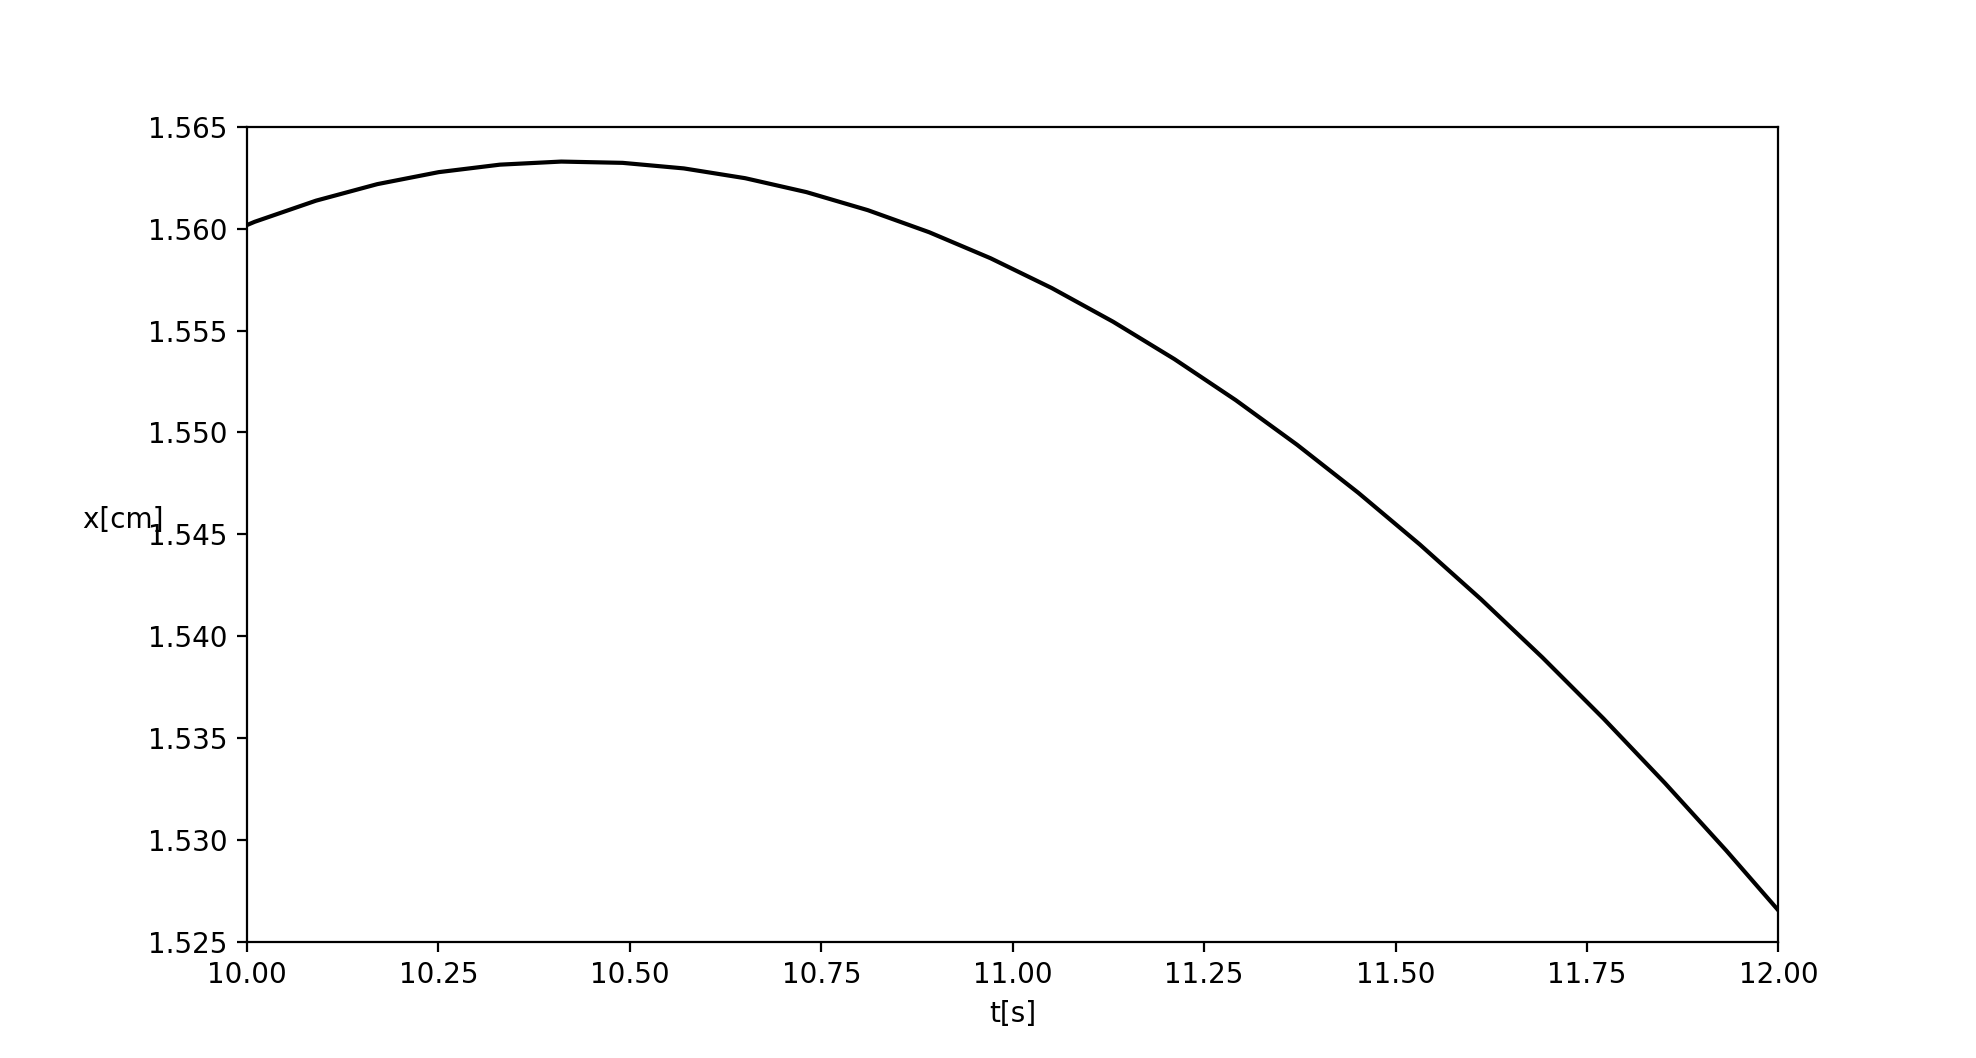
\includegraphics[width=15cm]{img/surp.png}
                \caption{$x(t)$のプロット($10\leq t \leq 12$)}
                \label{fig:surp}
            \end{figure}

            図では, $v_f(t) = 0$となる点である$t=10.426$付近で$x(t)$が
            極値を迎えている.
            このこととシミュレーション結果より, 数学的には$v_f(t)$が正しいが,
            実際の系では$v(t)$となることが予想される.

\section{天井クレーンの制御シミュレーション}
    この節では, 実験テキスト\cite{text}のFig.28に示されている天井クレーンのシミュレーションを行う.
    \subsection{吊り荷部の運動方程式}
        バネ-マス-ダンパ系のときと同様に,
        まずは吊り荷部の運動方程式をラグランジュ法を用いて導出する.

        吊り荷の$x$方向の変位を$x_l(t), y方向の変位をy_l(t)$とすると,

        \begin{eqnarray*}
            x_l(t) &=& x(t) + l\sin{\theta(t)} \\
            y_l(t) &=& l\cos{\theta(t)}
        \end{eqnarray*}

        となる. これらを$t$で微分することでそれぞれの方向の速度を出すことができる.
        
        \begin{eqnarray*}
            \dot{x_l}(t) &=& \dot{x}(t) + l\dot{\theta}(t)\cos{\theta(t)} \\
            \dot{y_l}(t) &=& -l\dot{\theta}(t)\sin{\theta(t)}
        \end{eqnarray*}

        吊り荷の速度を$v_l(t)$とすると, 以下のように表せる.

        \begin{eqnarray*}
            v_l(t)^2 &=& \dot{x_l}(t)^2 + \dot{y_l}(t)^2 \nonumber \\
            &=& \dot{x}(t)^2 + 2 l \dot{x}(t)\dot{\theta}(t)\cos{\theta(t)} + l^2 \dot{\theta}(t)^2
        \end{eqnarray*}

        これより, 吊り荷の運動エネルギーは,
        \[
            \frac{1}{2}mv_l(t)^2 = \frac{1}{2}m\{\dot{x}(t)^2 + 2 l \dot{x}(t)\dot{\theta}(t)\cos{\theta(t)} + l^2 \dot{\theta}(t)^2\}
        \]
        
        である. また, トロリーは$x$方向にのみ運動をするので,
        その運動エネルギーは$\displaystyle \frac{1}{2}M\dot{x}(t)^2$である.
        これらの和を取り, 系の運動エネルギー$T$は,

        \begin{equation}
            T = \frac{1}{2} m \{\dot{x}(t)^2 + 2 l \dot{x}(t)\dot{\theta}(t)\cos{\theta(t)} + l^2 \dot{\theta}(t)^2\} + \frac{1}{2}M\dot{x}(t)^2 \label{equ:t}
        \end{equation}

        となる.
        
        吊り荷の最下点を基準点とすると, 吊り荷の位置エネルギー$U$は,

        \begin{equation}
            U = mg\{l-y_l(t)\} = mgl\{1-\cos{\theta(t)}\} \label{equ:u}
        \end{equation}

        である.
        
        また, 散逸エネルギー$F$は次のようにできる.
        \begin{equation}
            F = \frac{1}{2} \mu \dot{\theta}(t)^2 \label{equ:f}
        \end{equation}

        ここで, ラグランジュの運動方程式方程式は次のように定義される.
    
        \begin{equation}
            \frac{d}{dt}\frac{\partial T}{\partial \dot{q_i}} - \frac{\partial T}{\partial q_i} + \frac{\partial U}{\partial q_i} + \frac{\partial F}{\partial \dot{q_i}} = \tau _i \label{equ:lag}
        \end{equation}
    
        $\tau _i$は物体に加わる外力であるが, 今回は0である.
        また, $q_i$は一般化座標といわれ, 今回は$q_i = \theta(t)$として計算をする.

        式(\ref{equ:t})より,

        \begin{eqnarray}
            \frac{d}{dt}\frac{\partial T}{\partial \dot{\theta}} &=& \frac{d}{dt}\frac{\partial}{\partial \dot{\theta}} \left(\frac{1}{2} m \{\dot{x}(t)^2 + 2 l \dot{x}(t)\dot{\theta}(t)\cos{\theta(t)} + l^2 \dot{\theta}(t)^2\} + \frac{1}{2}M\dot{x}(t)^2\right) \nonumber \\
            &=& \frac{d}{dt} ml\{\dot{x}(t)\cos{\theta(t)} + l\dot{\theta}(t)\} \nonumber \\
            &=& ml\{\ddot{x}(t)\cos{\theta(t)} - \dot{x}(t)\dot{\theta}(t)\sin{\theta(t)} + l\ddot{\theta}(t)\} \label{equ:ddt} \\
            \frac{\partial T}{\partial \theta} &=& \frac{\partial}{\partial \theta} \left(\frac{1}{2} m \{\dot{x}(t)^2 + 2 l \dot{x}(t)\dot{\theta}(t)\cos{\theta(t)} + l^2 \dot{\theta}(t)^2\} + \frac{1}{2}M\dot{x}(t)^2\right) \nonumber \\
            &=& -ml\dot{x}(t)\dot{\theta}(t)\sin{\theta(t)} \label{equ:dt}
        \end{eqnarray}

        式(\ref{equ:u})より,

        \begin{eqnarray}
            \frac{\partial U}{\partial \theta} &=& \frac{\partial}{\partial \theta} mgl\{1-\cos{\theta(t)}\} \nonumber \\
            &=& mgl\sin{\theta(t)} \label{equ:du}
        \end{eqnarray}

        式(\ref{equ:f})より,

        \begin{eqnarray}
            \frac{\partial F}{\partial \dot{\theta}} &=& \frac{\partial}{\partial \dot{\theta}} \frac{1}{2} \mu \dot{\theta}(t)^2 \nonumber \\
            &=& \mu \dot{\theta}(t) \label{equ:df}
        \end{eqnarray}

        となる.

        式(\ref{equ:lag})に式(\ref{equ:ddt}), (\ref{equ:dt}),
         (\ref{equ:du}), (\ref{equ:df}), $\tau _i = 0$を代入して,
        運動方程式は,

        \begin{eqnarray}
            ml\ddot{x}(t)\cos{\theta(t)} + ml^2\ddot{\theta}(t) + \mu \dot{\theta(t)} + mgl \sin{\theta(t)} &=& 0 \label{equ:trol}
        \end{eqnarray}
        
        となる.

    \subsection{パラメータの計算}
        シミュレーションをする際の定数として各値を計算する.
        各値は次のように与えられている.

        \begin{eqnarray*}
            m &=& 0.5 + \left(\frac{出席番号 - 25}{10}\right)^2 \ \mathrm{kg} \\
            l &=& 0.16 + 出席番号 \times 0.04 \ \mathrm{m} \\
            \mu &=& 1.22 \times 10^{-3} \ \mathrm{kg \cdot m^2 / s}
        \end{eqnarray*}

        私の出席番号は32であるので,
        これを代入して各値を計算すると,

        \begin{eqnarray*}
            m &=& 0.5 + \left(\frac{32 - 25}{10}\right)^2 = 0.99 \ \mathrm{kg} \\
            l &=& 0.16 + 32 \times 0.04 = 1.44 \ \mathrm{m} \\
        \end{eqnarray*}

        を得られる.

        これらを式(\ref{equ:trol})に代入すると,

        \[
            1.426\ddot{x}(t)\cos{\theta(t)} + 2.053\ddot{\theta}(t) + 1.22 \times 10^{-3} \dot{\theta(t)} + 13.97 \sin{\theta(t)} = 0
        \]

        となる.

    \subsection{PID制御器の設計とシミュレーション結果}
        PID制御とは目標値と制御量から操作量を決める制御方法である.
        今回はPID制御器を使ってシミュレーションを行う.

        PID制御器が扱う制御則は三つあり, 比例(Proportional)動作, 積分(Integral)動作, 微分(Derivative)動作である.
        それぞれ英語の頭文字がP, I, Dに対応している.

        比例動作は, 観測値と目標値の偏差に比例する制御則である.
        差が大きければ制御量も大きくし, そのまた逆も然りとする.

        積分動作は偏差の積分に比例する制御則である.
        これにより, 比例動作だけでは残ってしまう一定の偏差を取り除くことができる.

        微分動作は偏差の微分に比例する制御則である.
        これにより, 偏差の増減の動向を操作量に反映することができる.

        今回はサポートページ\cite{supp}にて配布されているシミュレーションモデルを使用して実験を進める.

        設計仕様として以下の二つが定められている.

        \begin{itemize}
            \item とろりは目標位置の印加後5s以内に整定し,
                オーバーシュートは5\%以内とする.
            \item 吊り荷の揺れ角は$\pm7^\circ$以内とする.
        \end{itemize}

        各パラメータでシミュレーションをした際の
        トロリの$x-t$グラフと吊り荷の$\theta - t$グラフをみながら
        これらを満たすようにトロリ, 吊り荷それぞれのPIDゲインを定めていく.
        なお, モデル内で与えられている初期値はトロリのPゲインが3で,
        他は全て0である.
        以下, トロリのPIDゲインを$P_t, I_t, D_t$, 吊り荷のPIDゲインを$P_l, I_l, D_l$とする.

        \subsubsection{Pゲインの調整}
            まずはじめに, Pゲインの調整を行う.
            二つのPゲインが動作にどのような影響を及ぼすのかをみるために,
            Pゲインのみを変化させながらシミュレーション結果をみてみる.
            
            \begin{figure}[h]
                \begin{minipage}{0.5\hsize}
                    \centering
                    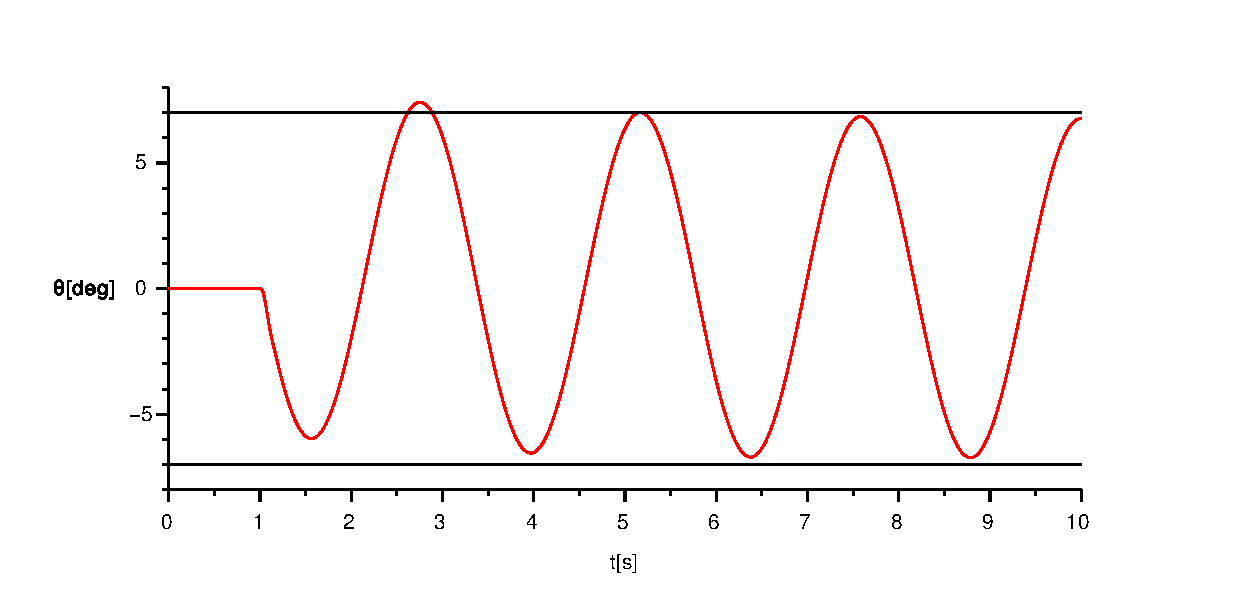
\includegraphics[width=9cm]{img/P5-0t.eps}
                \end{minipage}
                \begin{minipage}{0.5\hsize}
                    \centering
                    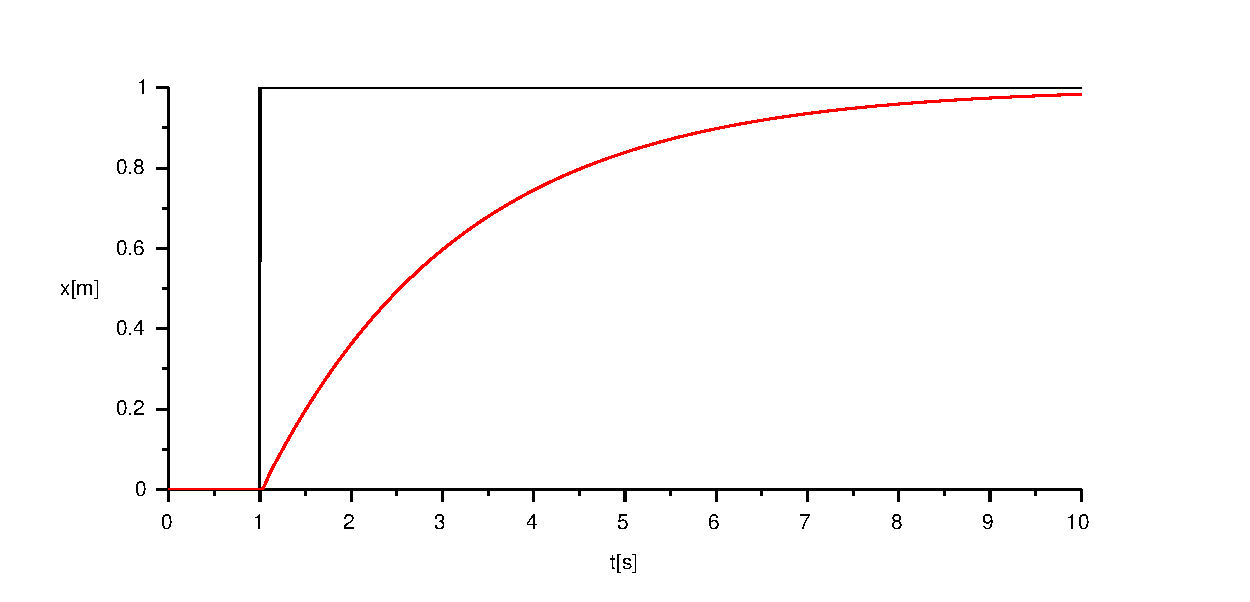
\includegraphics[width=9cm]{img/P5-0x.eps}
                \end{minipage}
                \caption{$P_t = 5, P_l = 0$のシミュレーション結果}
                \label{fig:p5-0}
            \end{figure}
            \begin{figure}[h]
                \begin{minipage}{0.5\hsize}
                    \centering
                    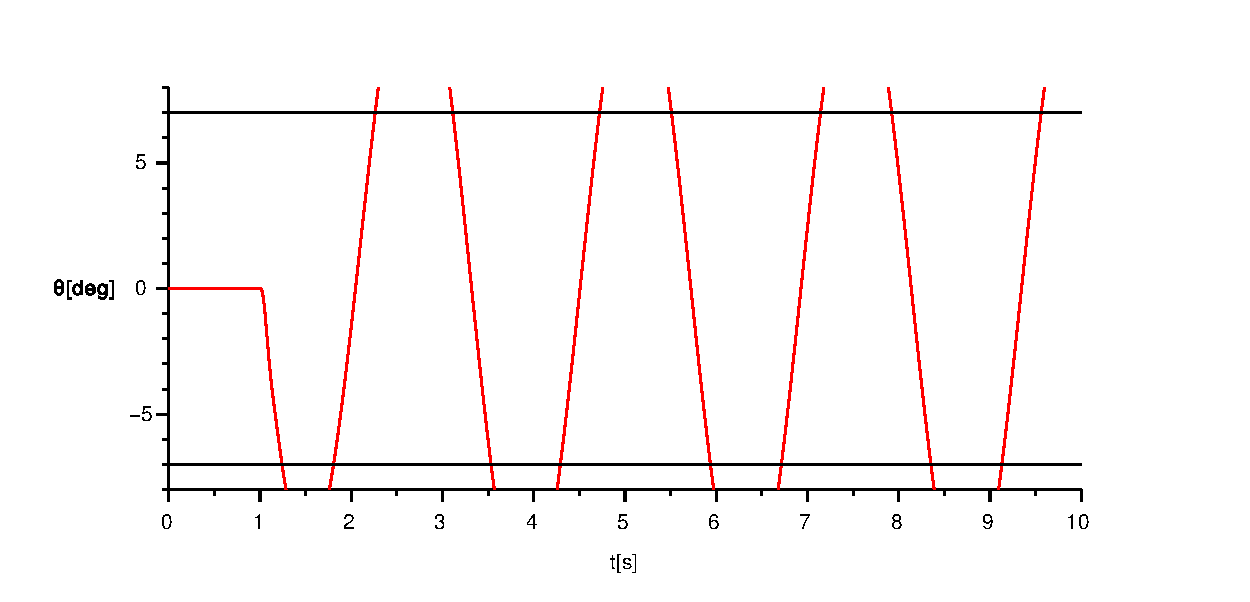
\includegraphics[width=9cm]{img/P10-0t.eps}
                \end{minipage}
                \begin{minipage}{0.5\hsize}
                    \centering
                    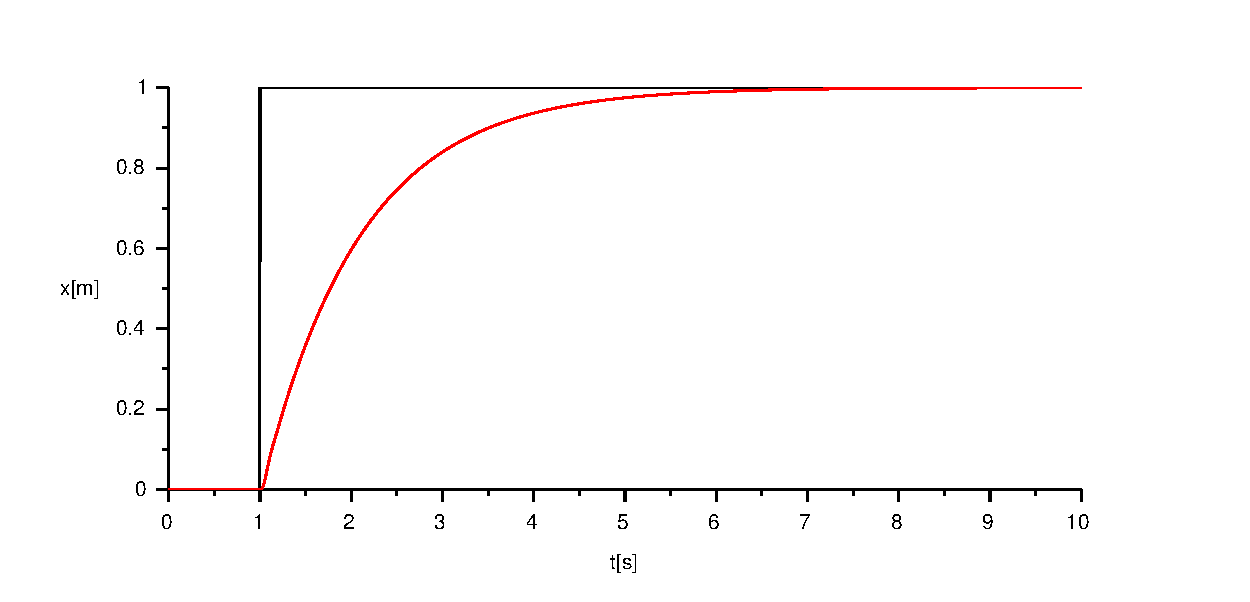
\includegraphics[width=9cm]{img/P10-0x.eps}
                \end{minipage}
                \caption{$P_t = 10, P_l = 0$のシミュレーション結果}
                \label{fig:p10-0}
            \end{figure}
            \begin{figure}[h]
                \begin{minipage}{0.5\hsize}
                    \centering
                    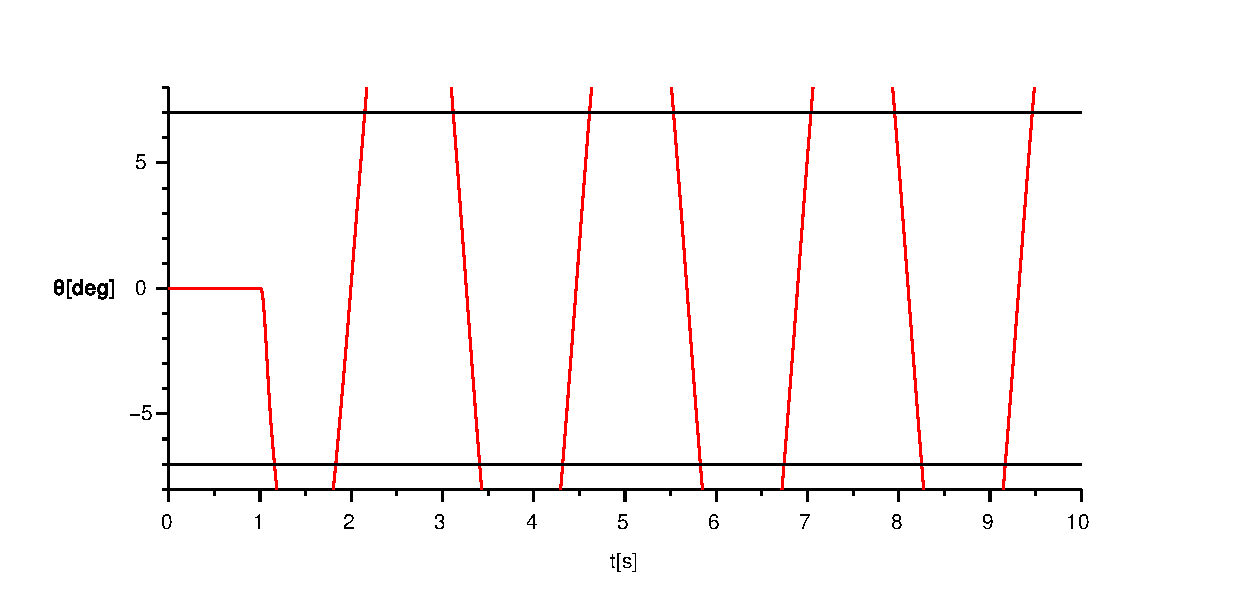
\includegraphics[width=9cm]{img/P15-0t.eps}
                \end{minipage}
                \begin{minipage}{0.5\hsize}
                    \centering
                    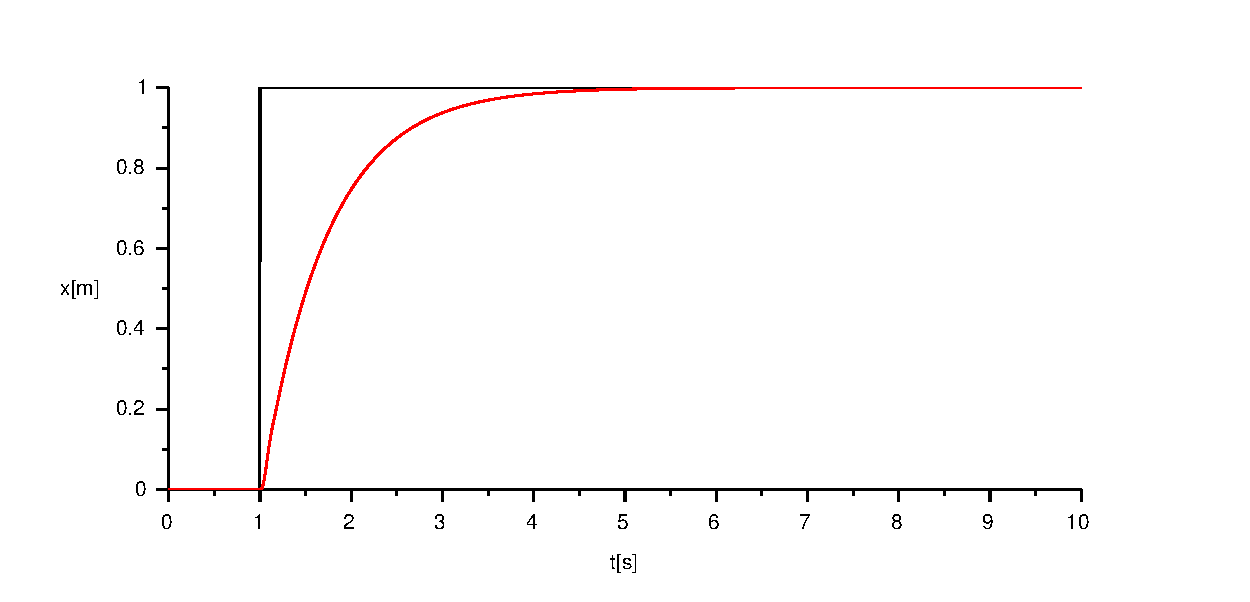
\includegraphics[width=9cm]{img/P15-0x.eps}
                \end{minipage}
                \caption{$P_t = 15, P_l = 0$のシミュレーション結果}
                \label{fig:p15-0}
            \end{figure}

            図\ref{fig:p5-0}, \ref{fig:p10-0}, \ref{fig:p15-0}は,
            $P_t$以外のパラメータを固定して,
            $P_t$を5, 10, 15と変化させたグラフである.
            グラフより, $P_t$が大きくなると, 吊り荷の揺れが大きくなり,
            トロリの整定が早まることがわかる.
            目標はトロリの整定がグラフ上で6秒以内であるので,
            ひとまず$P_t = 15$として調整を進める.

            \begin{figure}[h]
                \begin{minipage}{0.5\hsize}
                    \centering
                    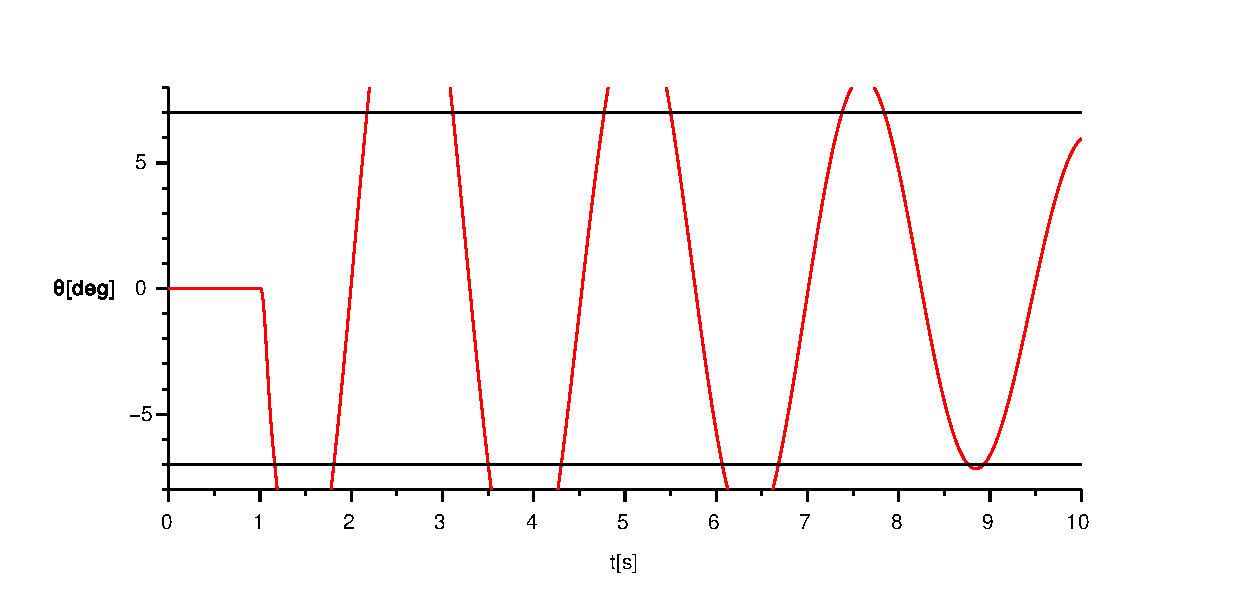
\includegraphics[width=9cm]{img/P15-5t.eps}
                \end{minipage}
                \begin{minipage}{0.5\hsize}
                    \centering
                    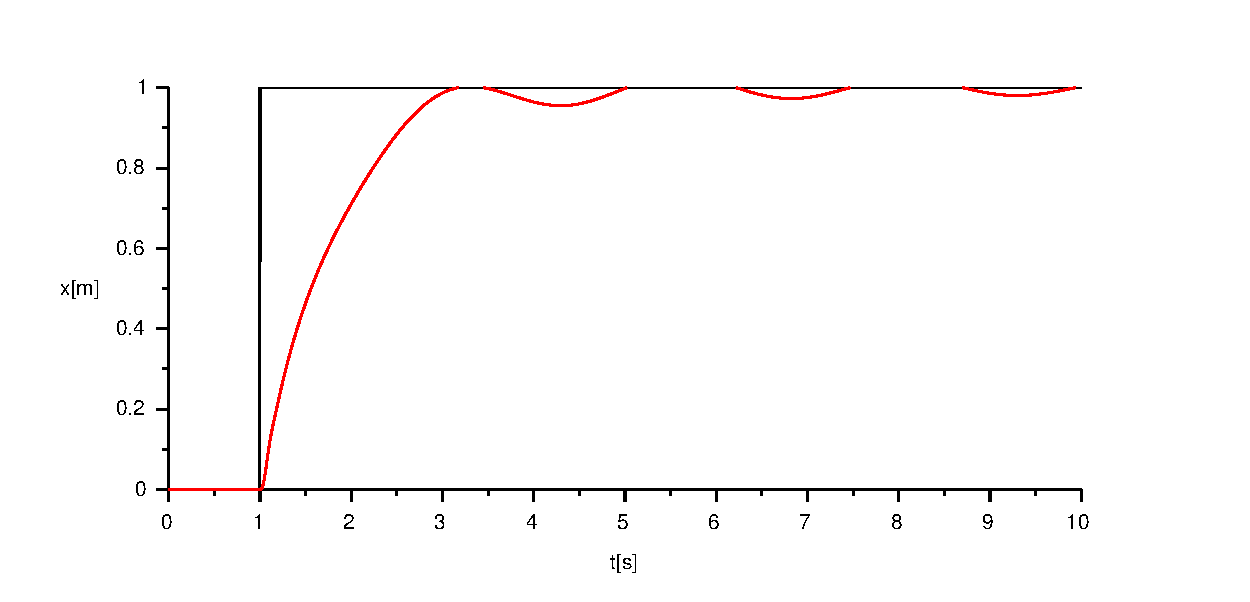
\includegraphics[width=9cm]{img/P15-5x.eps}
                \end{minipage}
                \caption{$P_t = 15, P_l = 5$のシミュレーション結果}
                \label{fig:p15-5}
            \end{figure}
            \begin{figure}[h]
                \begin{minipage}{0.5\hsize}
                    \centering
                    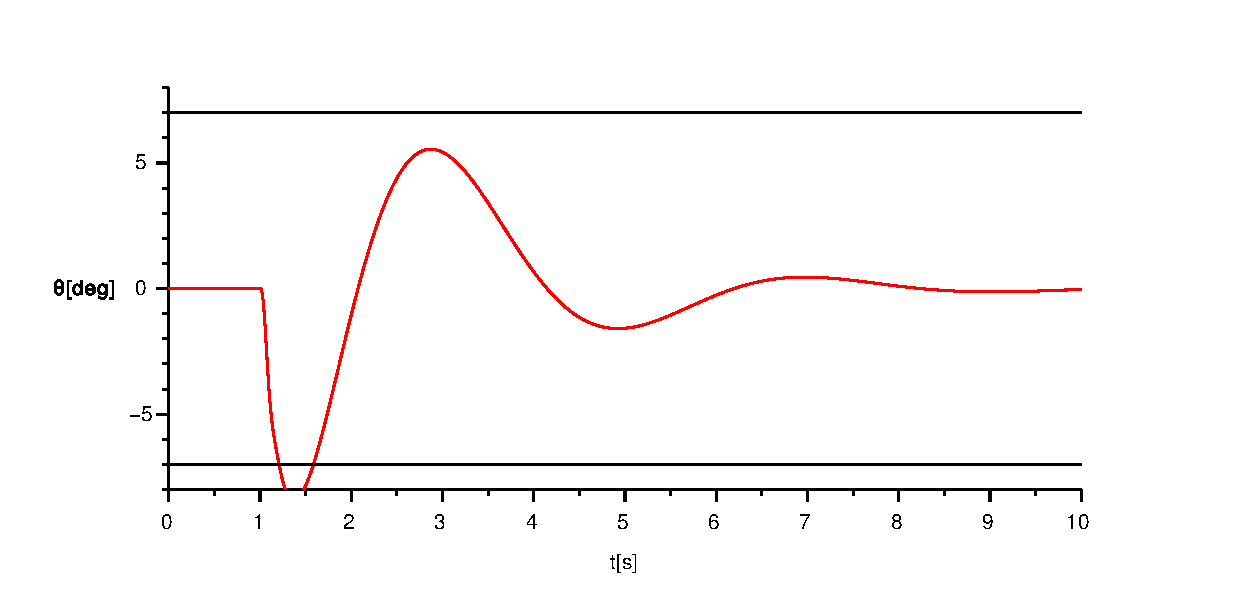
\includegraphics[width=9cm]{img/P15-50t.eps}
                \end{minipage}
                \begin{minipage}{0.5\hsize}
                    \centering
                    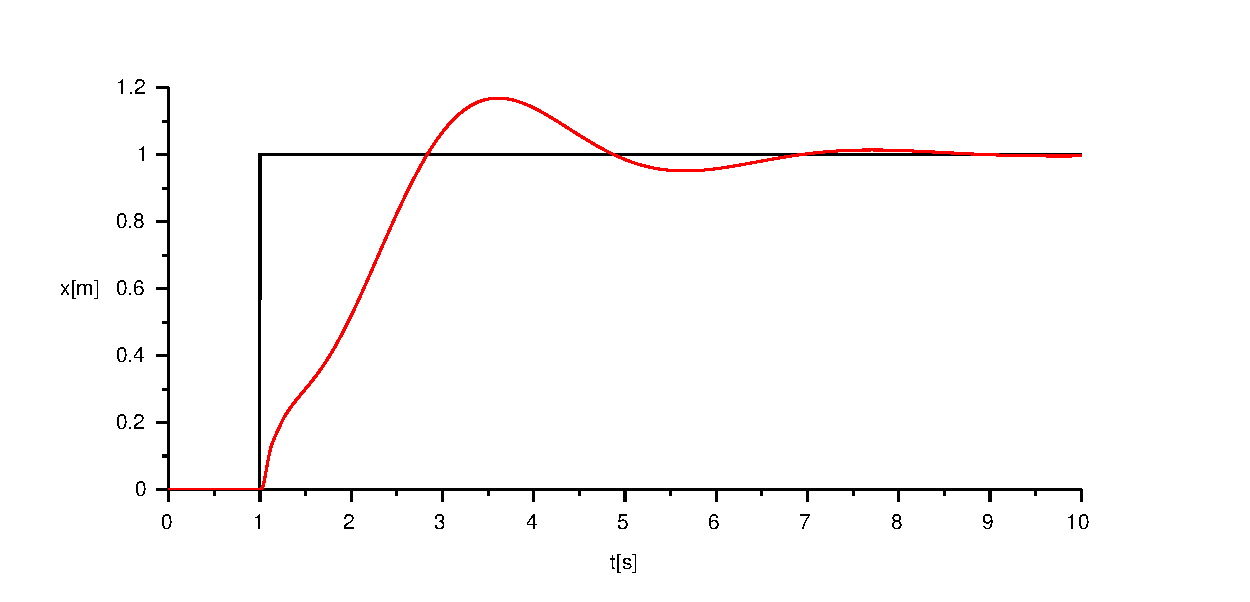
\includegraphics[width=9cm]{img/P15-50x.eps}
                \end{minipage}
                \caption{$P_t = 15, P_l = 50$のシミュレーション結果}
                \label{fig:p15-50}
            \end{figure}
            \begin{figure}[h]
                \begin{minipage}{0.5\hsize}
                    \centering
                    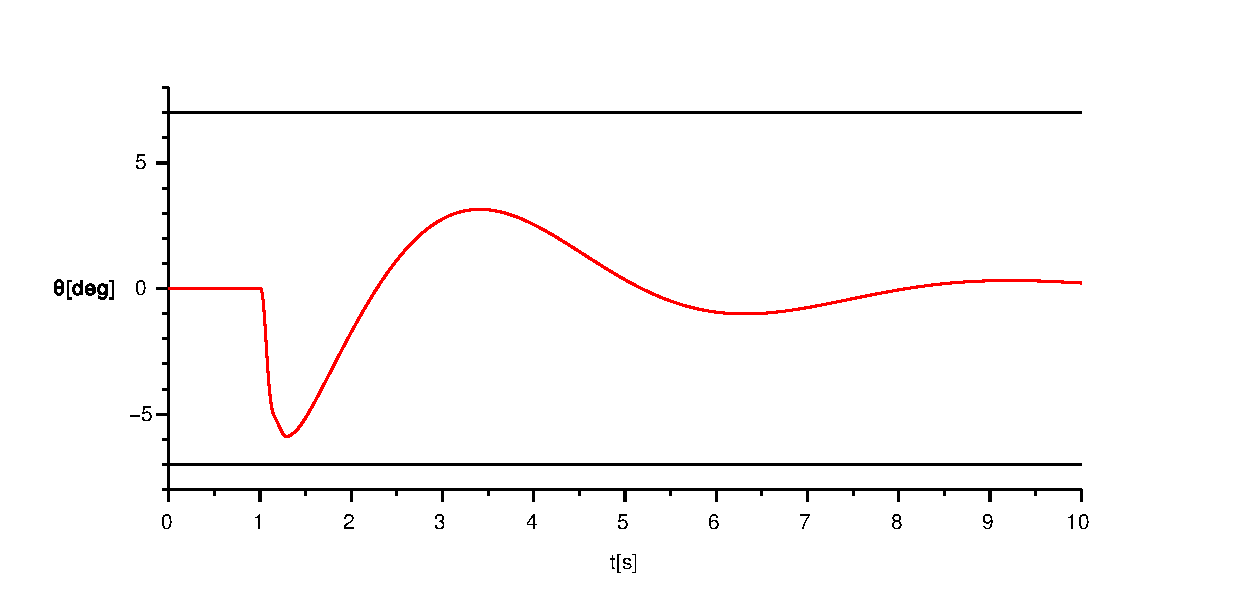
\includegraphics[width=9cm]{img/P15-100t.eps}
                \end{minipage}
                \begin{minipage}{0.5\hsize}
                    \centering
                    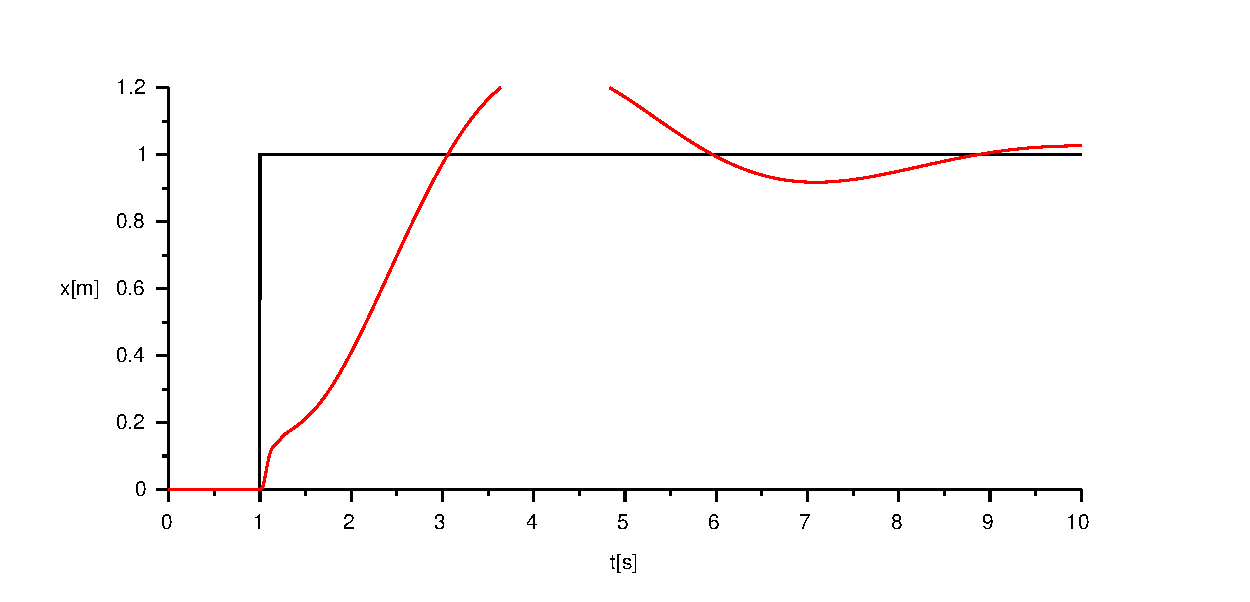
\includegraphics[width=9cm]{img/P15-100x.eps}
                \end{minipage}
                \caption{$P_t = 15, P_l = 100$のシミュレーション結果}
                \label{fig:p15-100}
            \end{figure}

            次に, 図\ref{fig:p15-5}, \ref{fig:p15-50}, \ref{fig:p15-100}は
            $P_l$のみを変化させたグラフである.
            $P_l$は大きくなると, 吊り荷の揺れが減り,
            トロリのオーバーシュートが大きくなることがわかる.
            トロリのオーバーシュートは5\%以内に収めなくてはいけないので,
            ひとまずは$P_l = 50$とする.

        \subsubsection{Iゲインの調整}
            次にIゲインによる制御を検証する.

            \begin{figure}[h]
                \begin{minipage}{0.5\hsize}
                    \centering
                    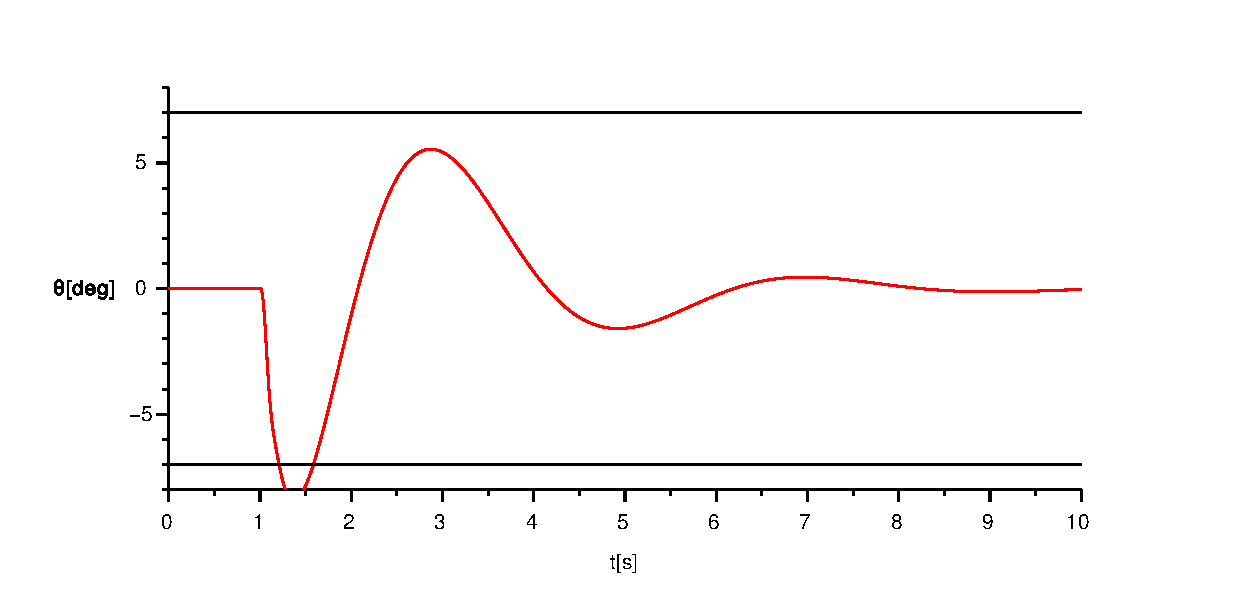
\includegraphics[width=9cm]{img/I0-0t.eps}
                \end{minipage}
                \begin{minipage}{0.5\hsize}
                    \centering
                    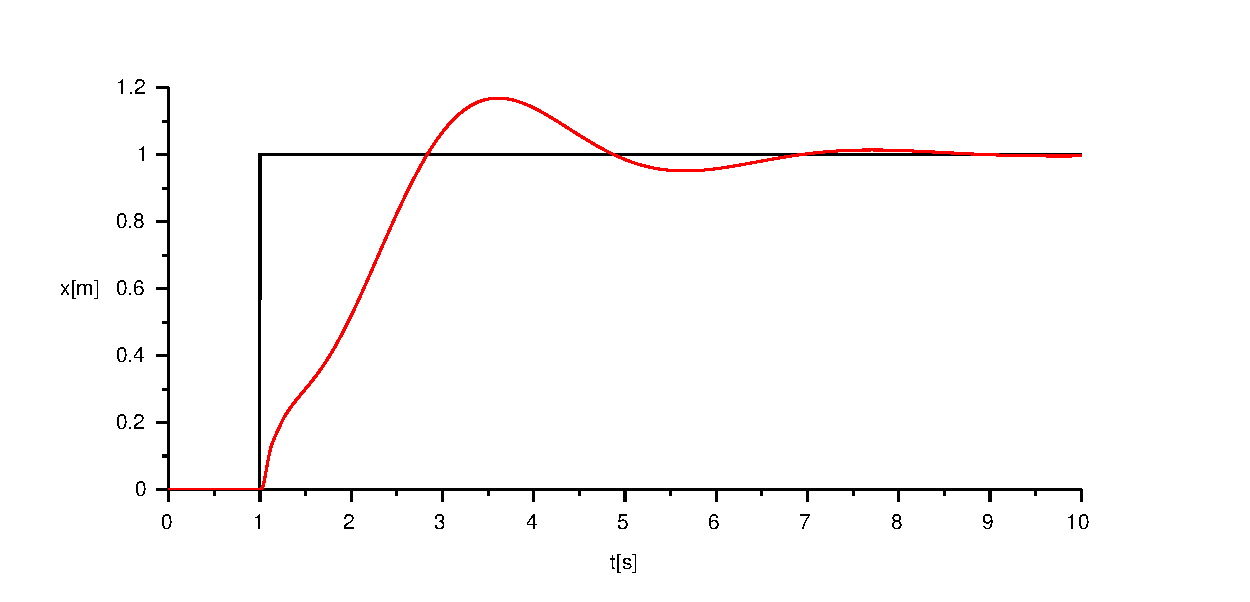
\includegraphics[width=9cm]{img/I0-0x.eps}
                \end{minipage}
                \caption{$I_t = 0, I_l = 0$のシミュレーション結果}
                \label{fig:i0-0}
            \end{figure}
            \begin{figure}[h]
                \begin{minipage}{0.5\hsize}
                    \centering
                    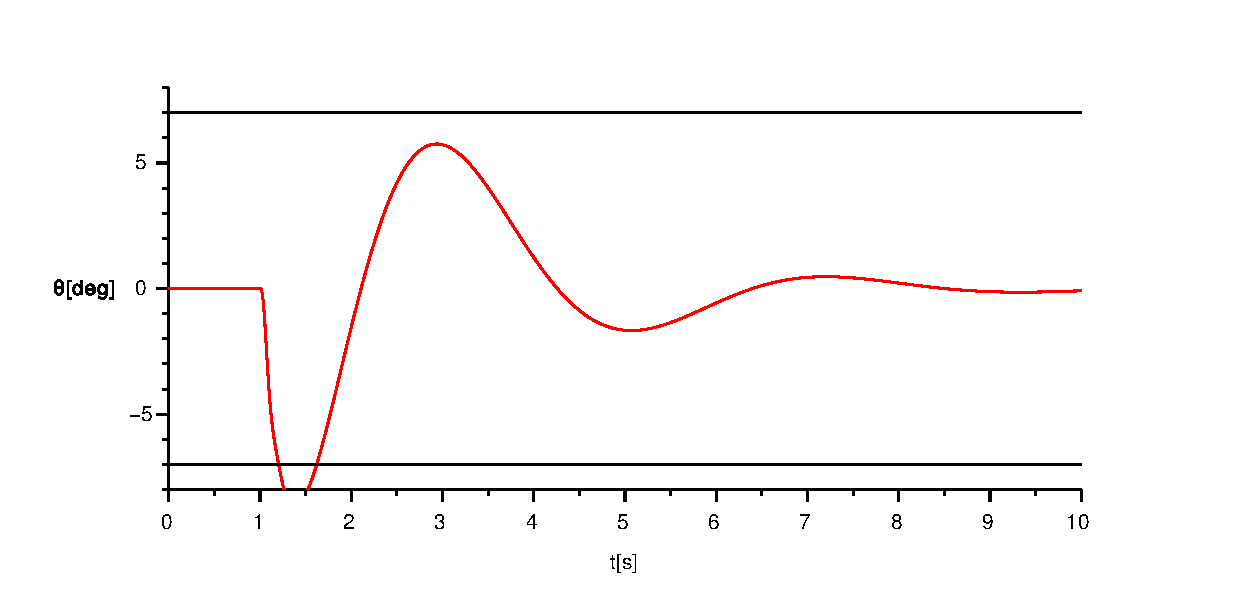
\includegraphics[width=9cm]{img/I2-0t.eps}
                \end{minipage}
                \begin{minipage}{0.5\hsize}
                    \centering
                    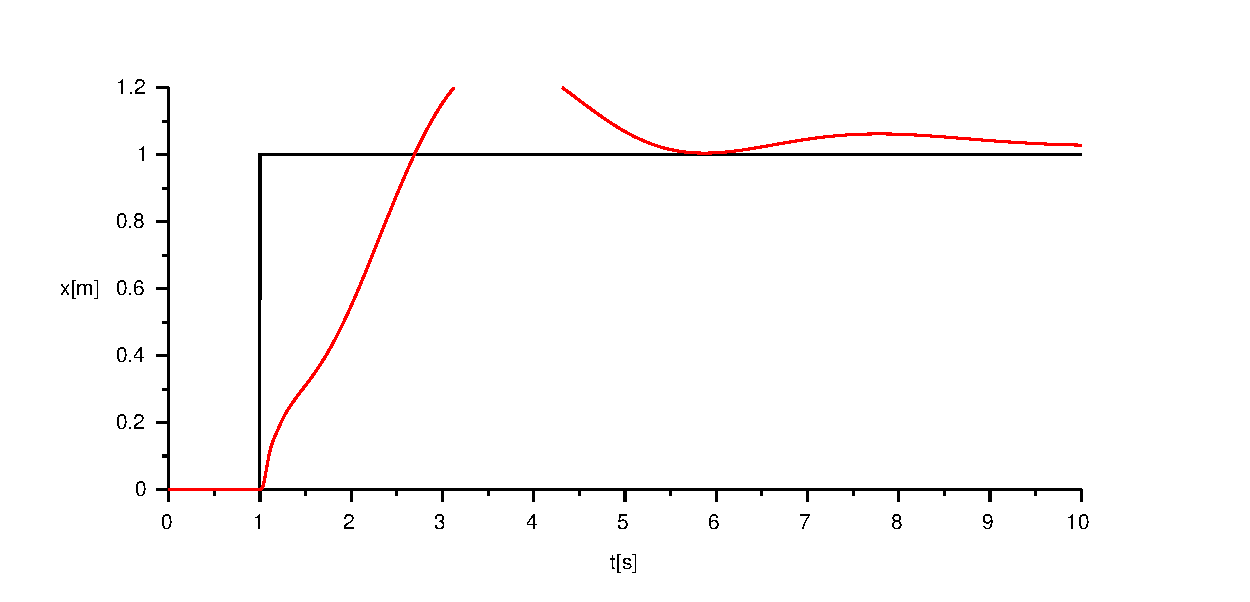
\includegraphics[width=9cm]{img/I2-0x.eps}
                \end{minipage}
                \caption{$I_t = 2, I_l = 0$のシミュレーション結果}
                \label{fig:i2-0}
            \end{figure}
            \begin{figure}[h]
                \begin{minipage}{0.5\hsize}
                    \centering
                    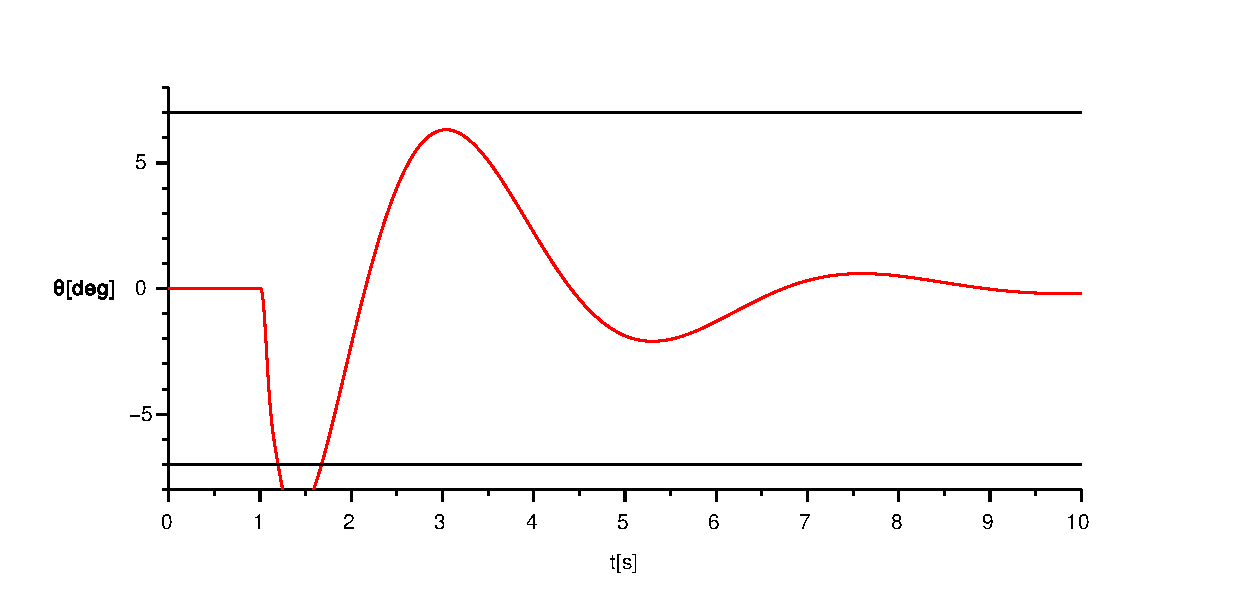
\includegraphics[width=9cm]{img/I5-0t.eps}
                \end{minipage}
                \begin{minipage}{0.5\hsize}
                    \centering
                    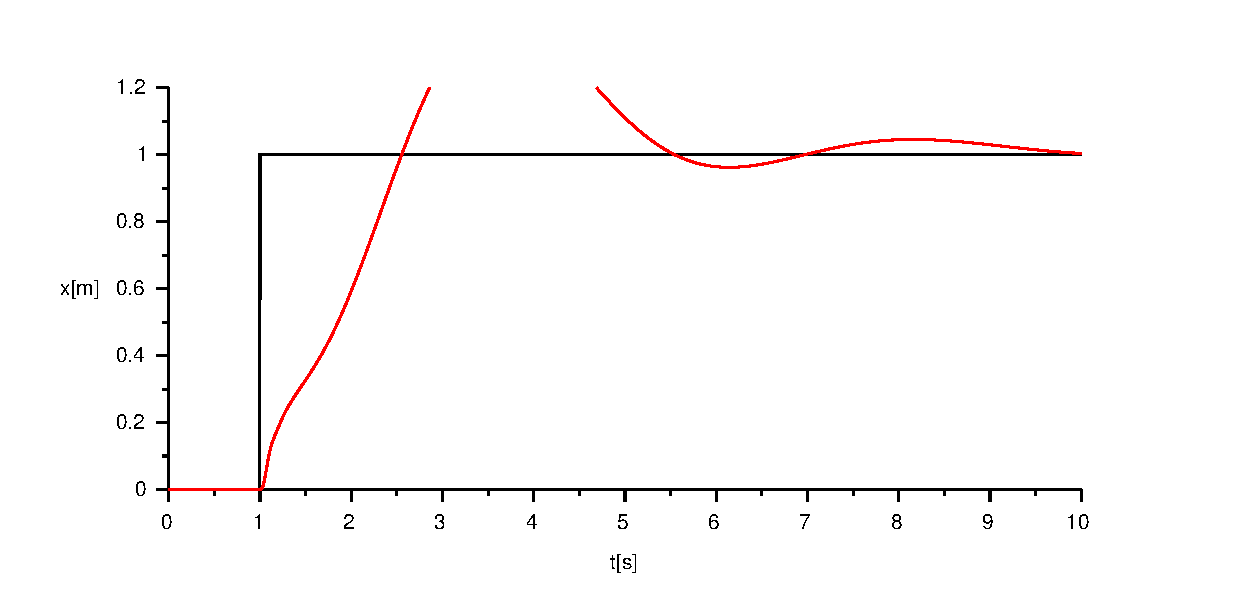
\includegraphics[width=9cm]{img/I5-0x.eps}
                \end{minipage}
                \caption{$I_t = 5, I_l = 0$のシミュレーション結果}
                \label{fig:i5-0}
            \end{figure}

            図\ref{fig:i0-0}, \ref{fig:i2-0}, \ref{fig:i5-0}は
            $I_t$のみを変化させたグラフである.
            $I_t$が大きくなると, 吊り荷の挙動は変化せずに,
            トロリのオーバーシュートが大きくなっていることがわかる.
            今回のシミュレーションではオーバーシュートは必要ないので,
            $I_t = 0$として検証を進める.

            \begin{figure}[h]
                \begin{minipage}{0.5\hsize}
                    \centering
                    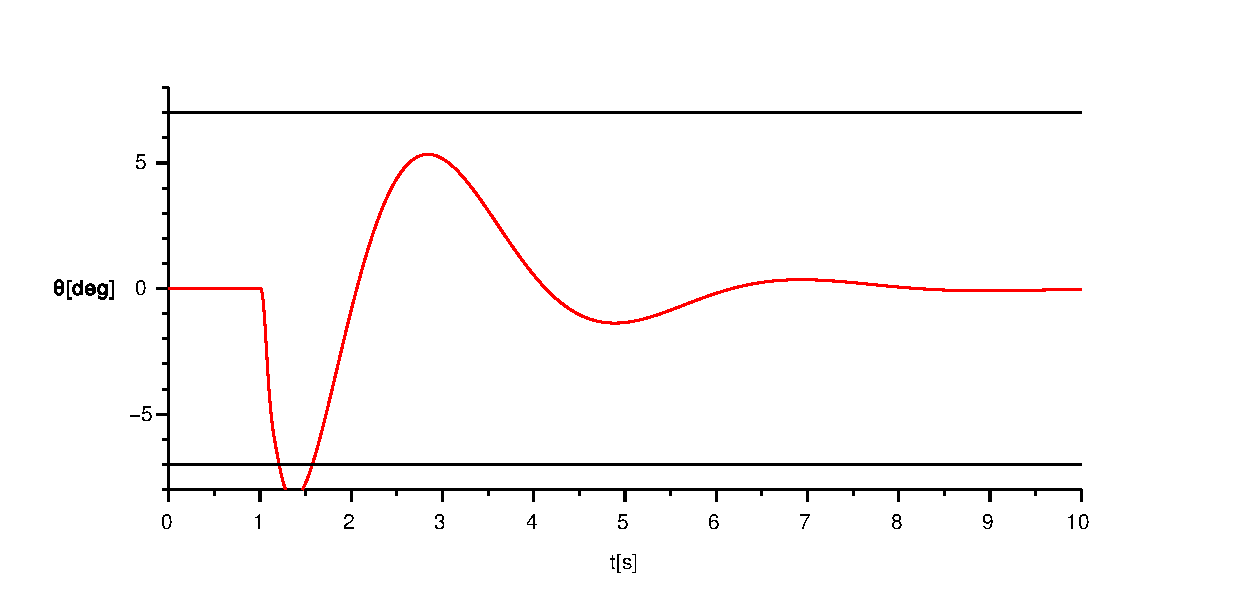
\includegraphics[width=9cm]{img/I0-5t.eps}
                \end{minipage}
                \begin{minipage}{0.5\hsize}
                    \centering
                    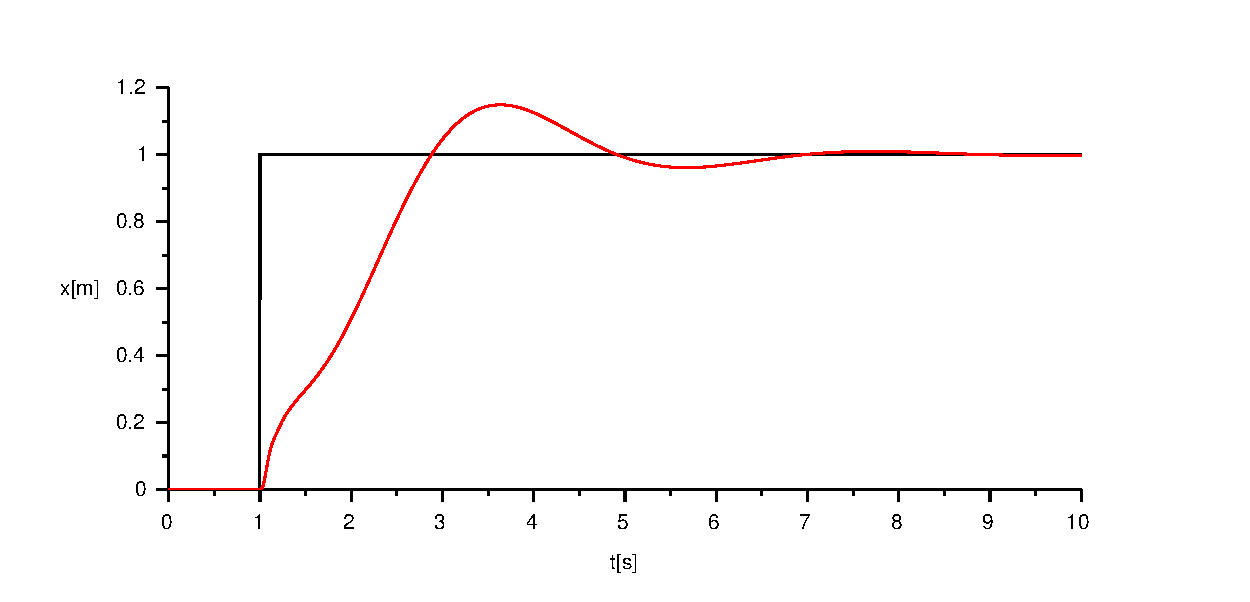
\includegraphics[width=9cm]{img/I0-5x.eps}
                \end{minipage}
                \caption{$I_t = 0, I_l = 5$のシミュレーション結果}
                \label{fig:i0-5}
            \end{figure}
            \begin{figure}[h]
                \begin{minipage}{0.5\hsize}
                    \centering
                    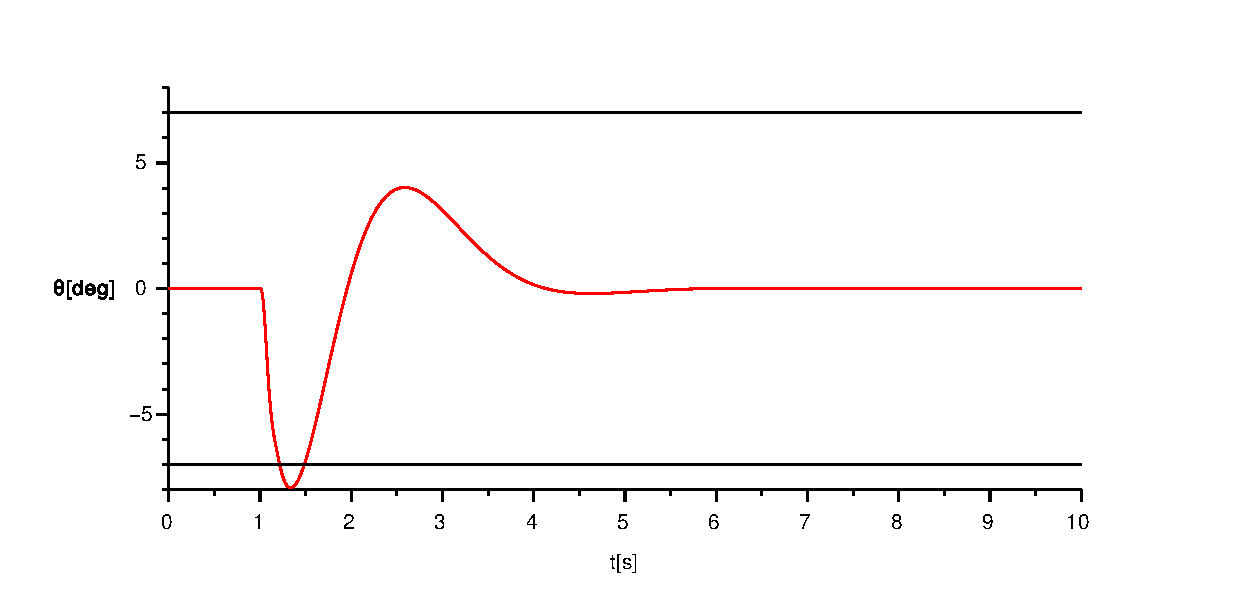
\includegraphics[width=9cm]{img/I0-50t.eps}
                \end{minipage}
                \begin{minipage}{0.5\hsize}
                    \centering
                    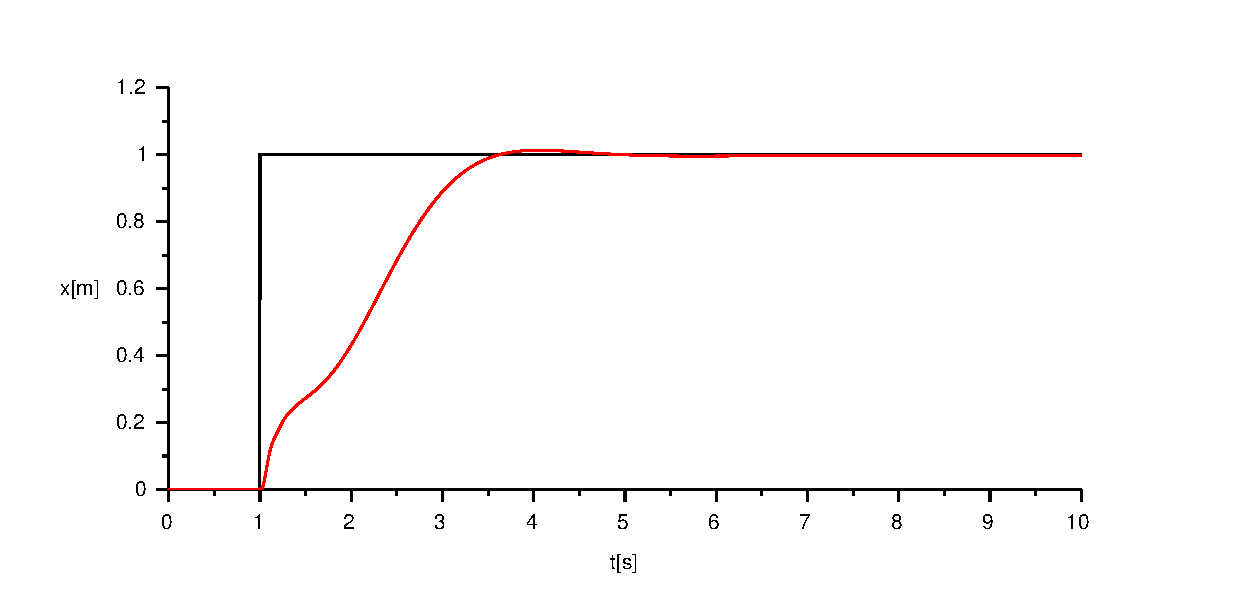
\includegraphics[width=9cm]{img/I0-50x.eps}
                \end{minipage}
                \caption{$I_t = 0, I_l = 50$のシミュレーション結果}
                \label{fig:i0-50}
            \end{figure}
            \begin{figure}[h]
                \begin{minipage}{0.5\hsize}
                    \centering
                    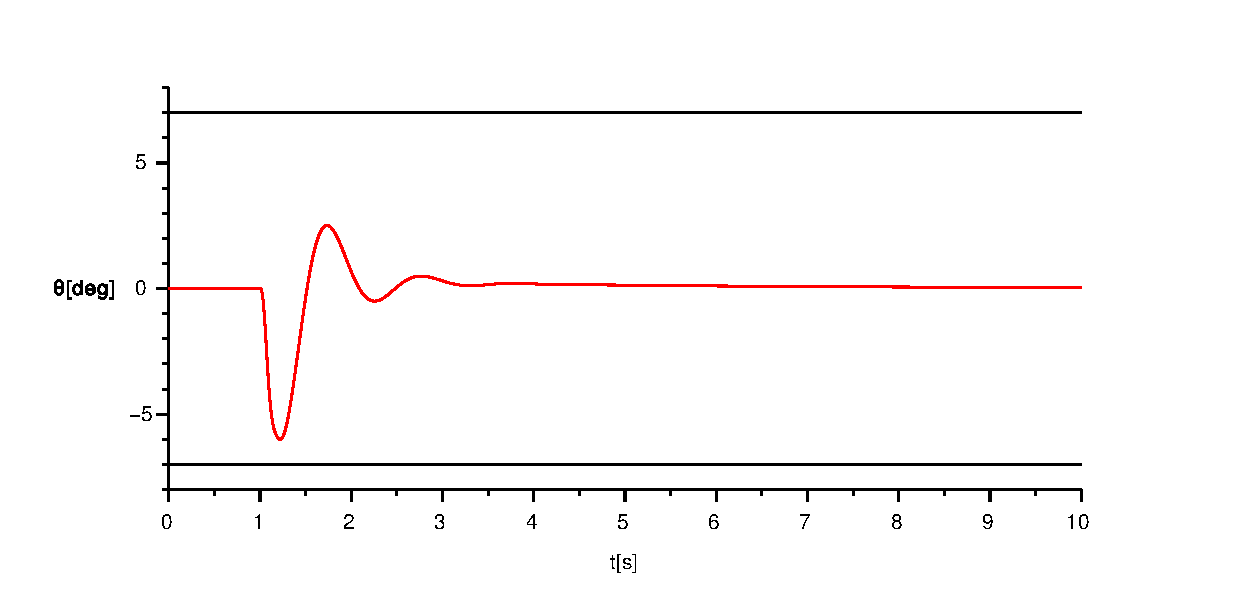
\includegraphics[width=9cm]{img/I0-500t.eps}
                \end{minipage}
                \begin{minipage}{0.5\hsize}
                    \centering
                    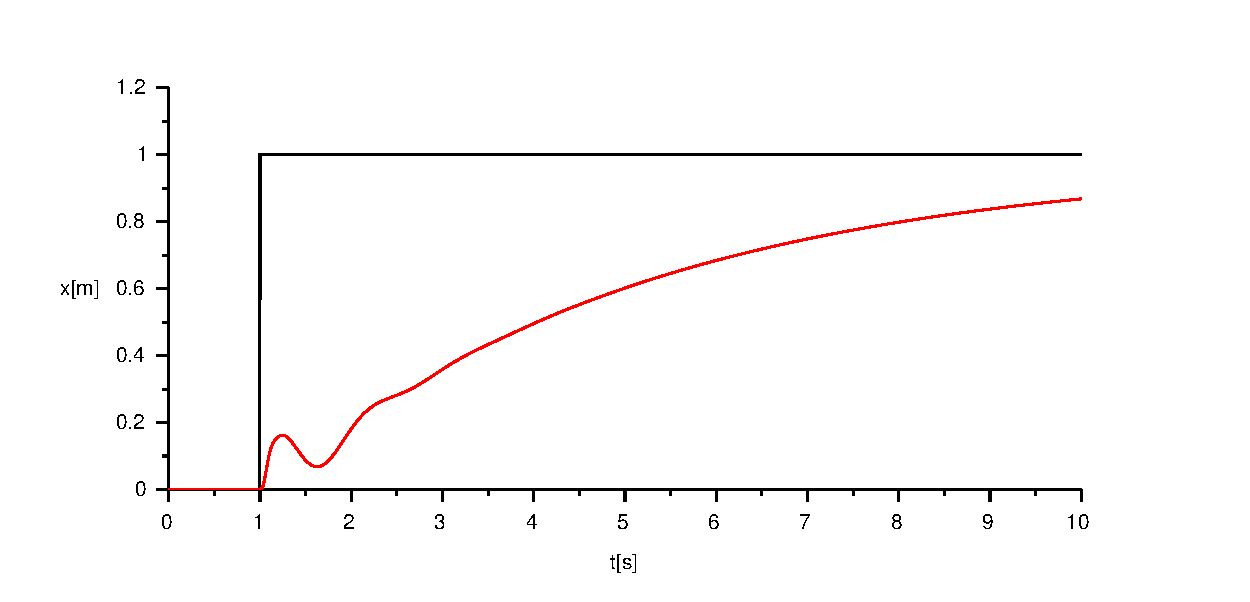
\includegraphics[width=9cm]{img/I0-500x.eps}
                \end{minipage}
                \caption{$I_t = 0, I_l = 500$のシミュレーション結果}
                \label{fig:i0-500}
            \end{figure}

            次に図\ref{fig:i0-5}, \ref{fig:i0-50}, \ref{fig:i0-500}
            は$I_l$のみを変化させたグラフである.
            $I_l$が増加すると吊り荷の振幅が抑えられ,
            トロリのオーバーシュートが抑えられるが,
            大きくしすぎると図\ref{fig:i0-500}のように整定が著しく遅くなってしまう.
            $I_l = 50$として検証を進める.

        \subsubsection{Dゲインの調整}
            最後に, Dゲインの働きをみる.

            \begin{figure}[h]
                \begin{minipage}{0.5\hsize}
                    \centering
                    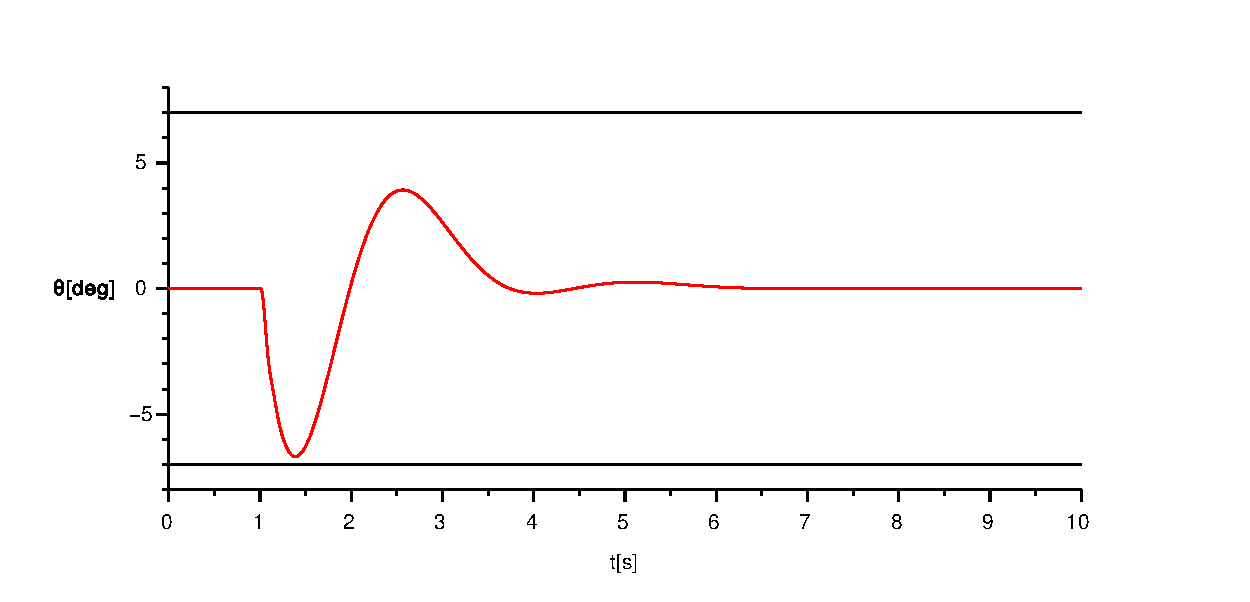
\includegraphics[width=9cm]{img/D5-0t.eps}
                \end{minipage}
                \begin{minipage}{0.5\hsize}
                    \centering
                    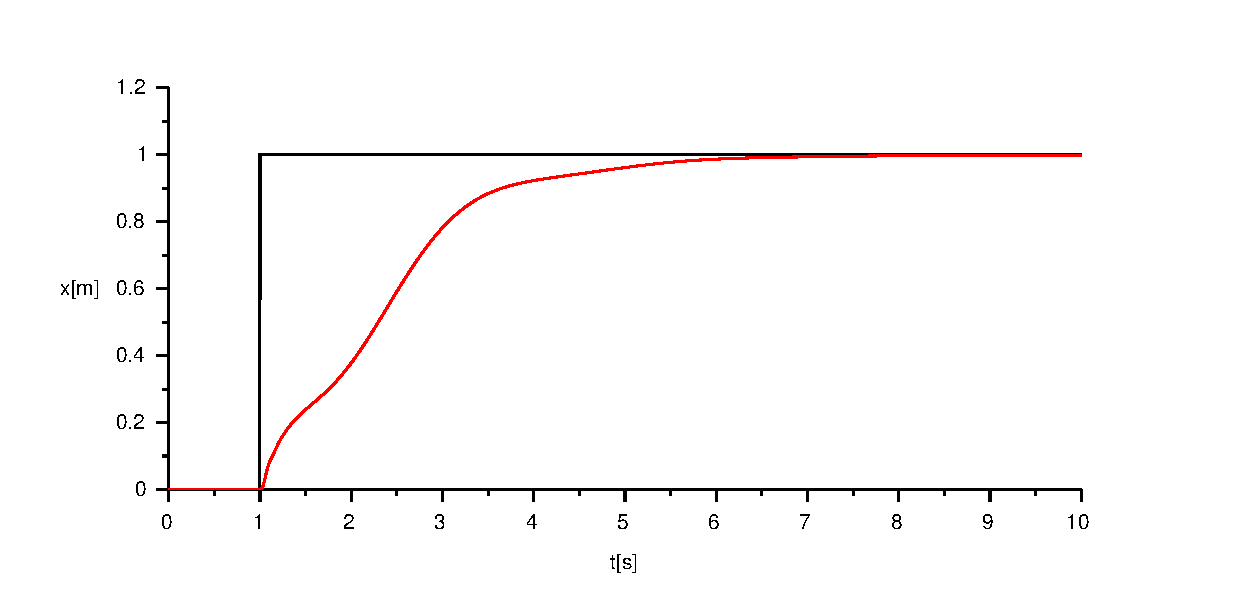
\includegraphics[width=9cm]{img/D5-0x.eps}
                \end{minipage}
                \caption{$D_t = 5, D_l = 0$のシミュレーション結果}
                \label{fig:d5-0}
            \end{figure}
            \begin{figure}[h]
                \begin{minipage}{0.5\hsize}
                    \centering
                    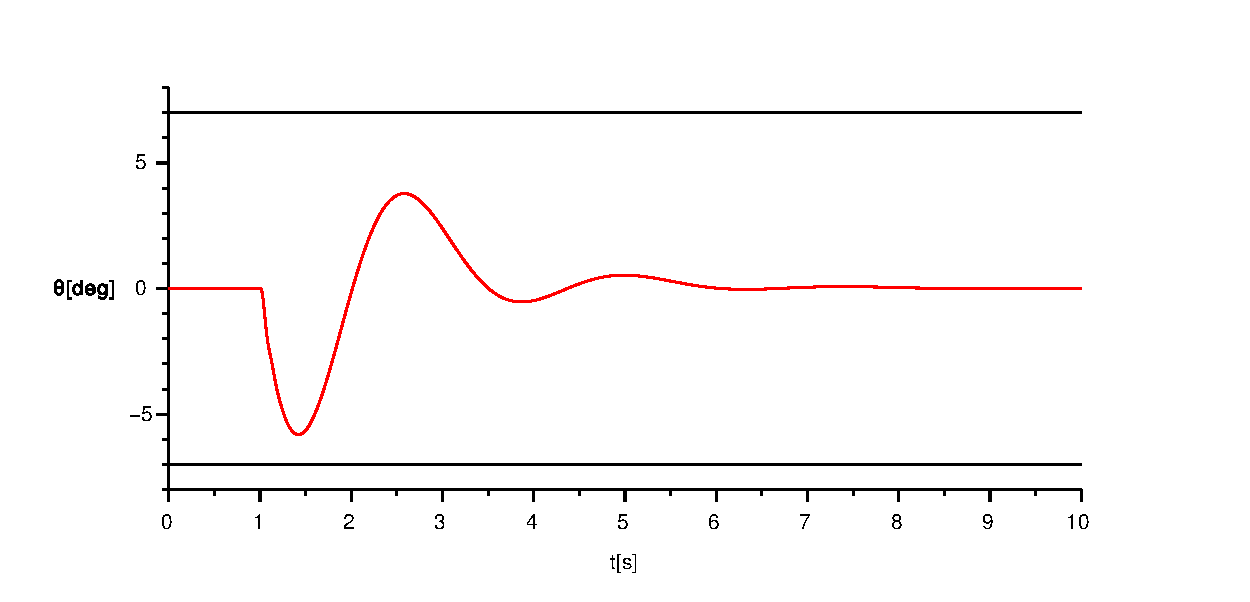
\includegraphics[width=9cm]{img/D10-0t.eps}
                \end{minipage}
                \begin{minipage}{0.5\hsize}
                    \centering
                    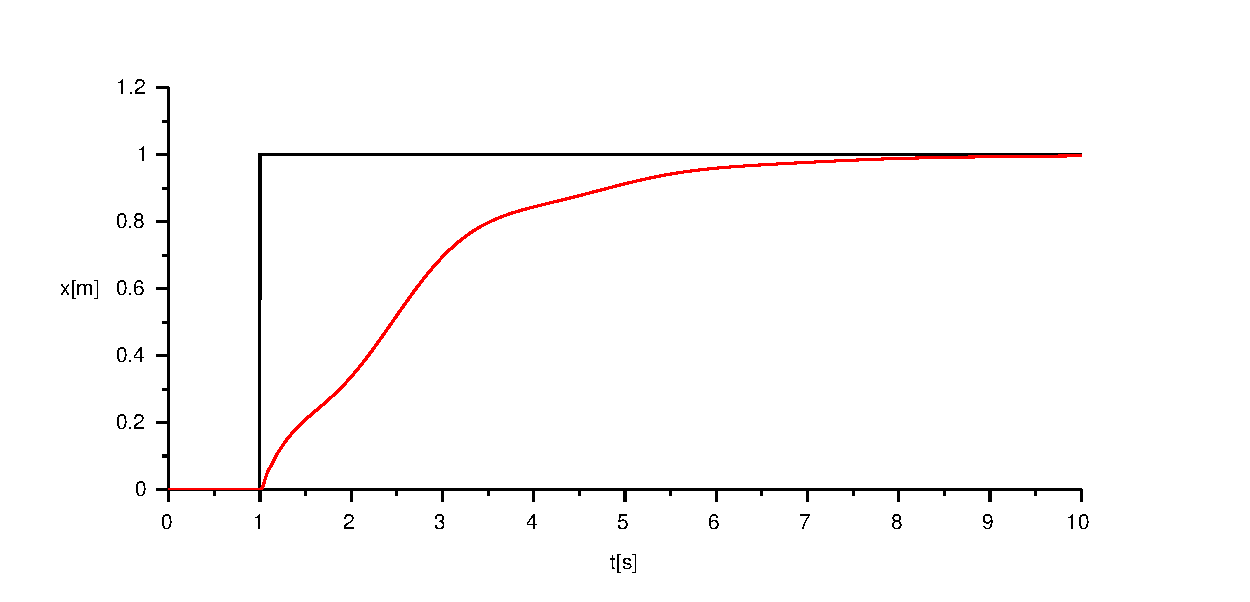
\includegraphics[width=9cm]{img/D10-0x.eps}
                \end{minipage}
                \caption{$D_t = 10, D_l = 0$のシミュレーション結果}
                \label{fig:d10-0}
            \end{figure}
            \begin{figure}[h]
                \begin{minipage}{0.5\hsize}
                    \centering
                    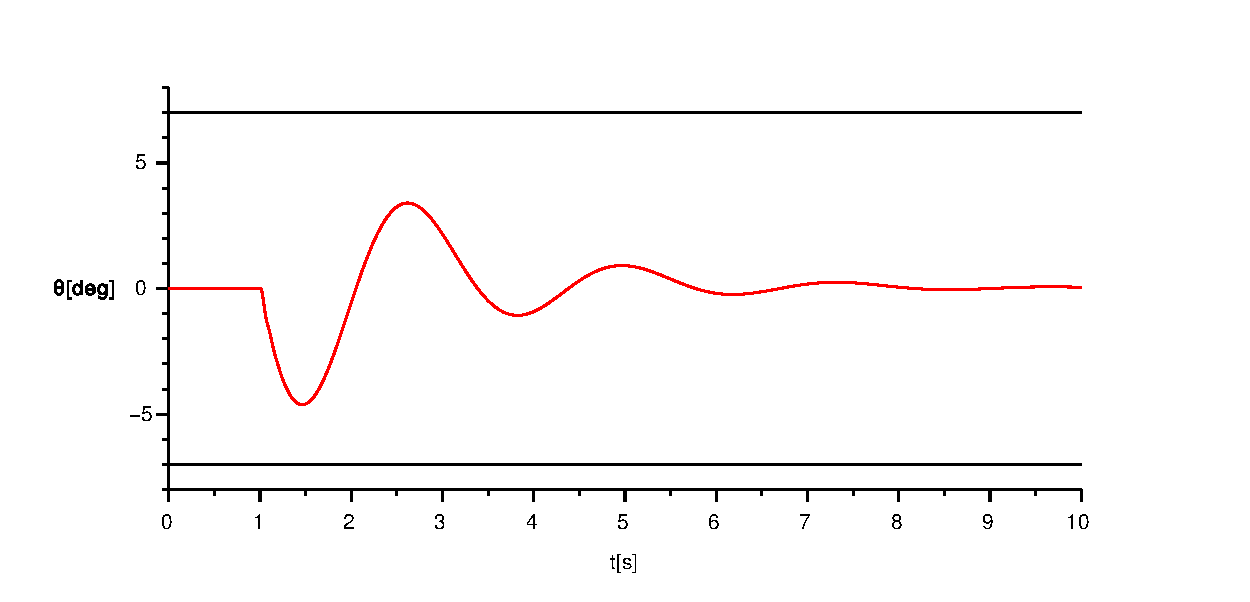
\includegraphics[width=9cm]{img/D20-0t.eps}
                \end{minipage}
                \begin{minipage}{0.5\hsize}
                    \centering
                    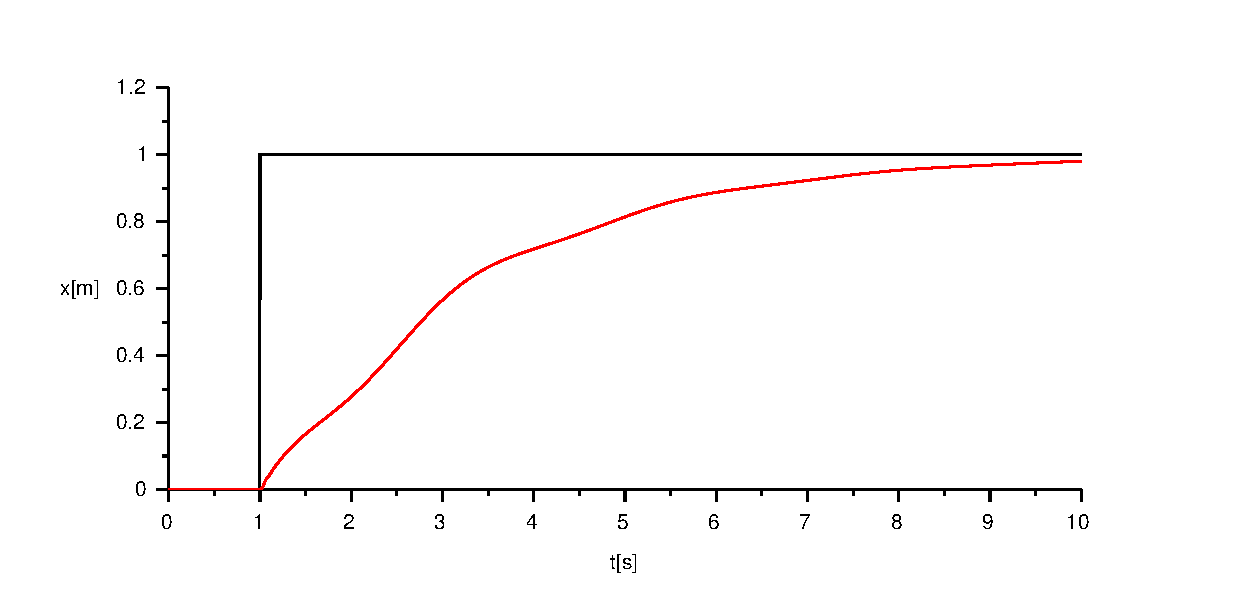
\includegraphics[width=9cm]{img/D20-0x.eps}
                \end{minipage}
                \caption{$D_t = 20, D_l = 0$のシミュレーション結果}
                \label{fig:d20-0}
            \end{figure}

            図\ref{fig:d5-0}, \ref{fig:d10-0}, \ref{fig:d20-0}
            は$D_t$のみを変化させたグラフである.
            $D_t$が大きくなると吊り荷の振動,
            トロリの変位ともに小さくなることがわかる.
            現状ではトロリの変位が小さくなってしまうと整定が間に合わないので,
            $D_t = 5$とする.

            \begin{figure}[h]
                \begin{minipage}{0.5\hsize}
                    \centering
                    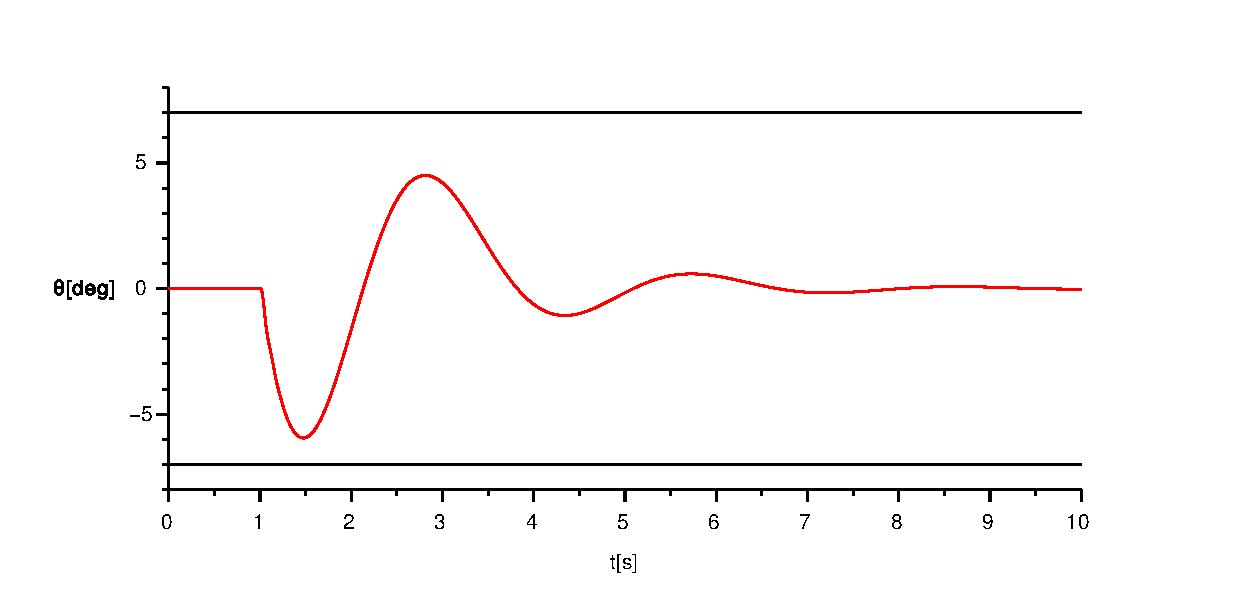
\includegraphics[width=9cm]{img/D5-10t.eps}
                \end{minipage}
                \begin{minipage}{0.5\hsize}
                    \centering
                    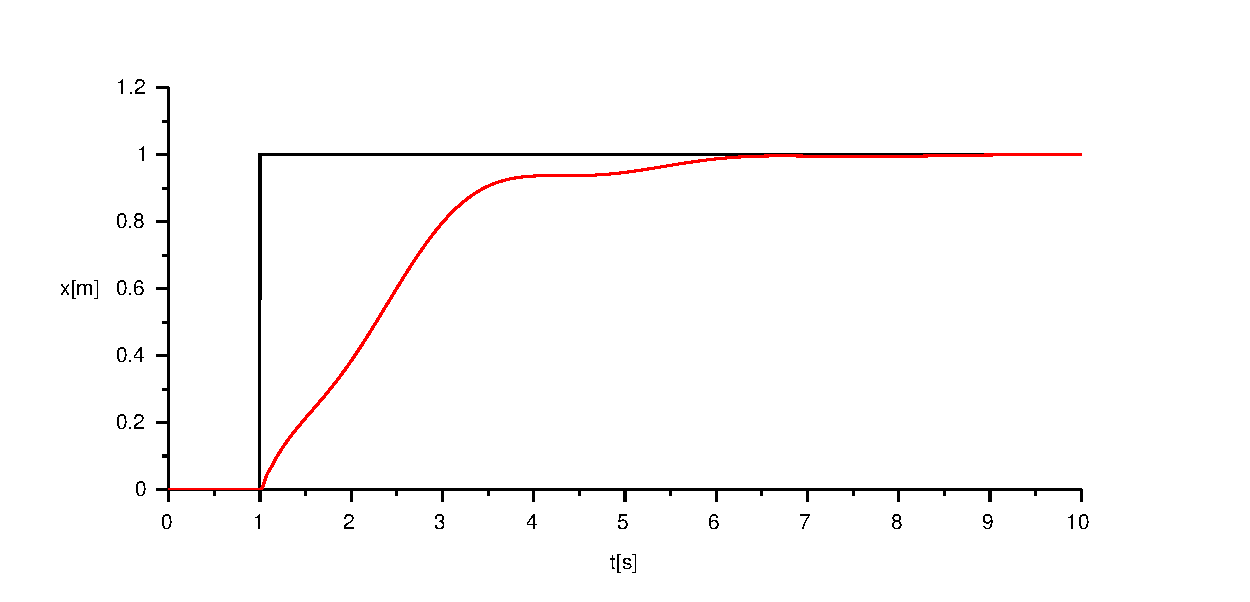
\includegraphics[width=9cm]{img/D5-10x.eps}
                \end{minipage}
                \caption{$D_t = 5, D_l = 10$のシミュレーション結果}
                \label{fig:d5-10}
            \end{figure}
            \begin{figure}[h]
                \begin{minipage}{0.5\hsize}
                    \centering
                    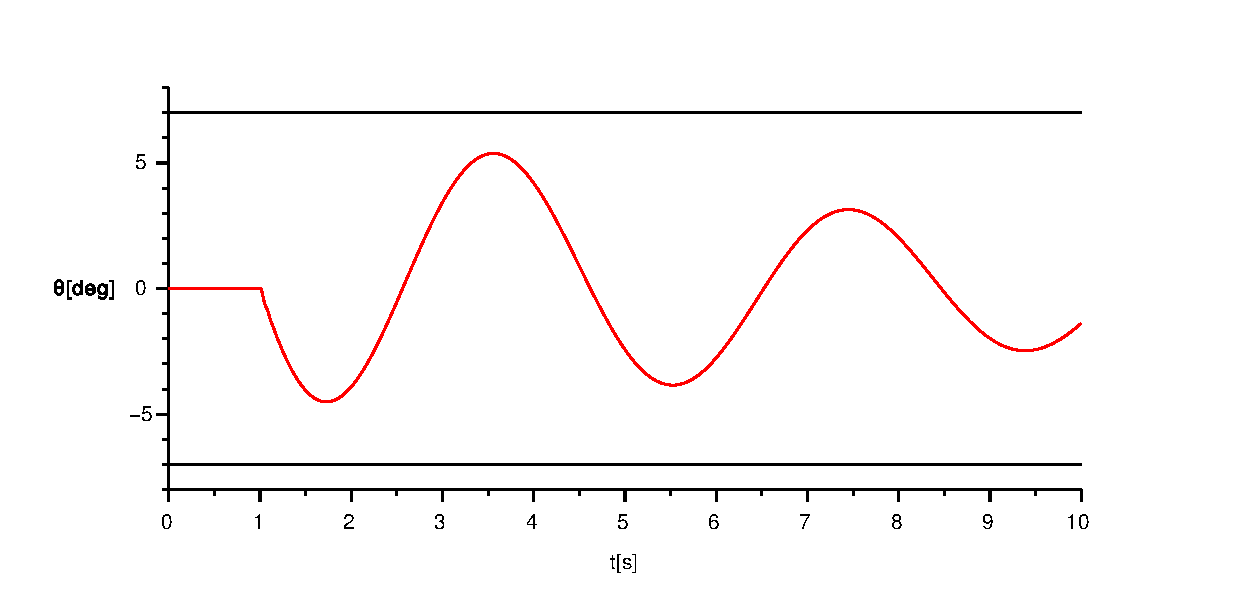
\includegraphics[width=9cm]{img/D5-50t.eps}
                \end{minipage}
                \begin{minipage}{0.5\hsize}
                    \centering
                    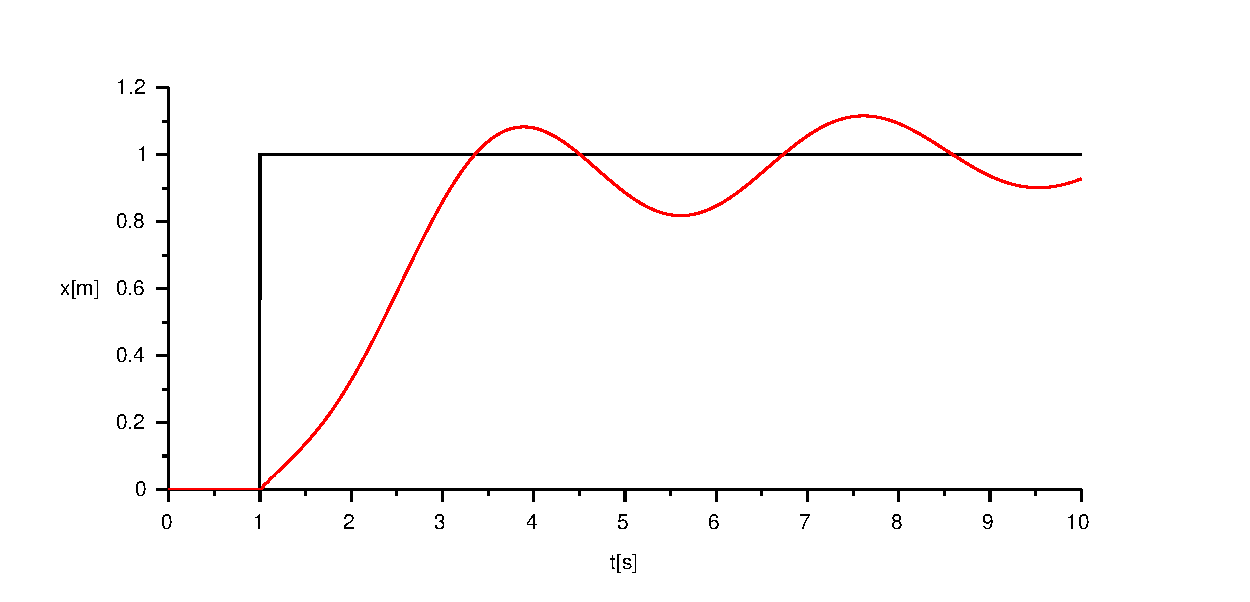
\includegraphics[width=9cm]{img/D5-50x.eps}
                \end{minipage}
                \caption{$D_t = 5, D_l = 50$のシミュレーション結果}
                \label{fig:d5-50}
            \end{figure}

            最後に, 図\ref{fig:d5-0}, 図\ref{fig:d5-10}, 図\ref{fig:d5-50}
            は$D_l$のみ変化させたグラフである.
            $D_l$が大きくなると, 吊り荷の振動, トロリの変位ともに大きくなり,
            振動回数が増えてしまうことがわかる.
            ひとまず$D_l = 0$とする.

        \subsubsection{ゲインの確定}
            ここまでで各ゲインがクレーンの応答に及ぼす影響がわかったので,
            これらを踏まえて値を確定する.

            試行錯誤の結果, 表\ref{tab:gain}に示すように値を定めた.

            \begin{table}[h]
                \caption{最終的なゲインの値}
                \label{tab:gain}
                \centering
                \begin{tabular}{c||c|c|c}
                    & P & I & D \\ \hline \hline
                    トロリ & 30 & 0 & 30 \\ \hline
                    吊り荷 & 200 & 29 & 0
                \end{tabular}
            \end{table}

            この値を用いてシミュレーションを行った結果を図\ref{fig:king}に示す.

            \begin{figure}[h]
                \begin{minipage}{0.5\hsize}
                    \centering
                    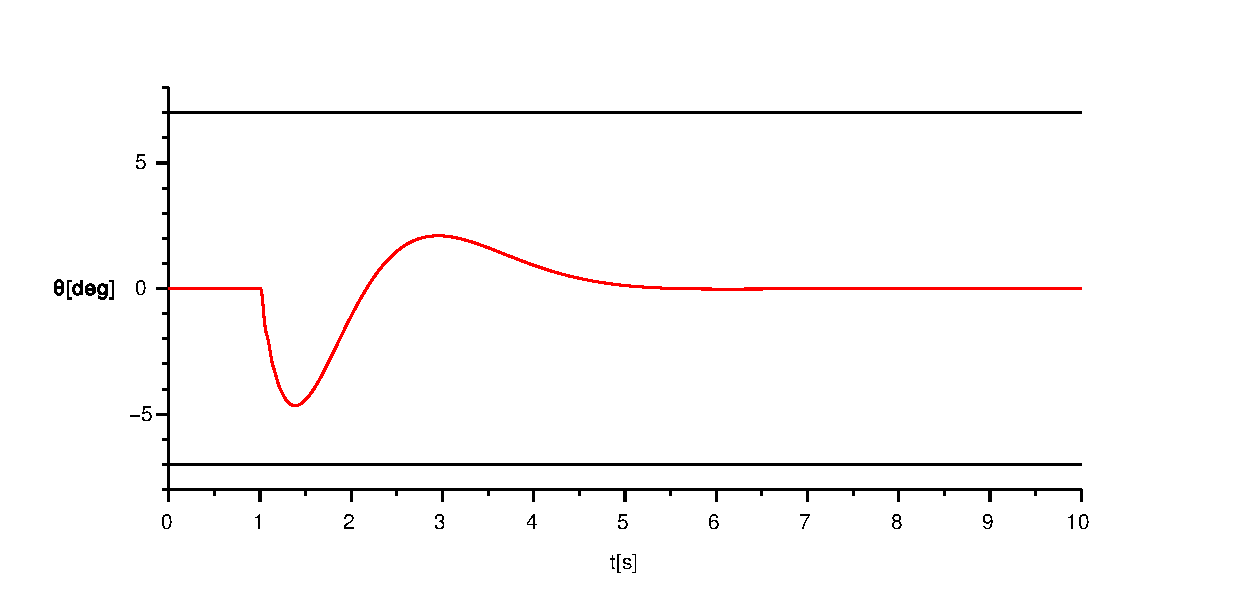
\includegraphics[width=9cm]{img/kingt.eps}
                \end{minipage}
                \begin{minipage}{0.5\hsize}
                    \centering
                    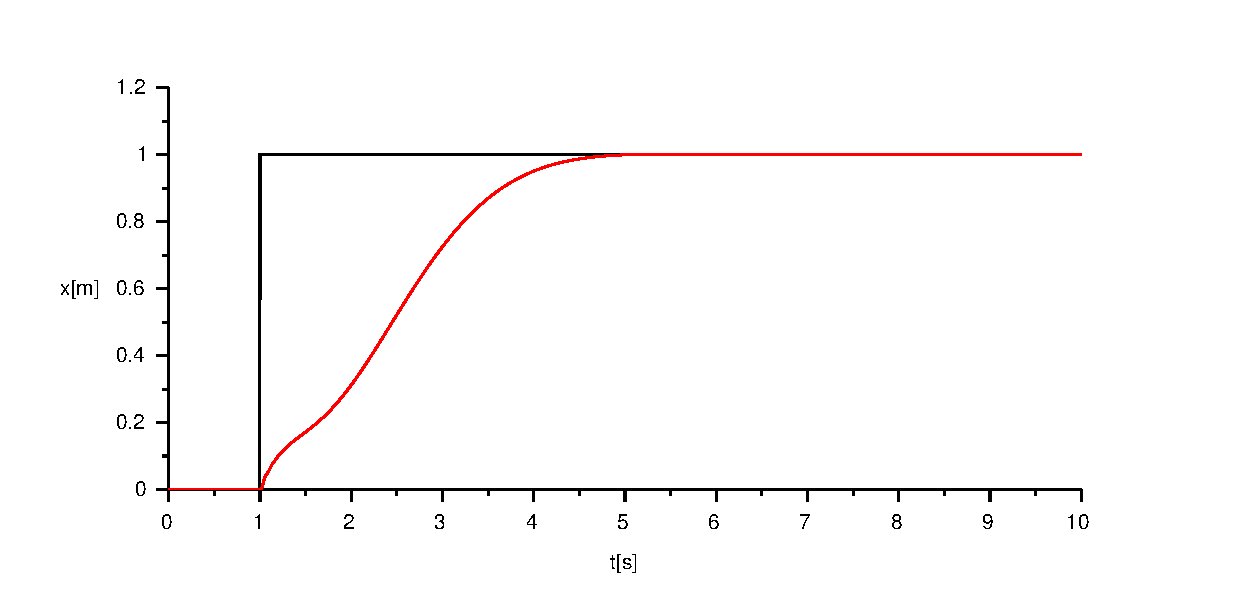
\includegraphics[width=9cm]{img/kingx.eps}
                \end{minipage}
                \caption{最終的なシミュレーション結果}
                \label{fig:king}
            \end{figure}

            図より, 二つの設計仕様を満たしていることがわかる.

\section{感想}
    案の定, 水曜日(締め切り前々日)にレポートを書き始めることとなってしまった.
    怠惰を招いた原因として,
    普段使っているMacではScilabの一部機能がうまく動かなかったことがある.
    私はMatlabのライセンスを所持しているのでそちらで同時にシミュレーションを確認しながら
    実験を進めた.

    結果としてレポートを書き終えることができたが,
    今後は今までのように時間に余裕を持って進めていきたい.

\begin{thebibliography}{99}
    \bibitem{text} 数値シミュレーション, 電子制御工学実験$\cdot$ 4年後期テキスト, 2020
    \bibitem{supp} 数値シミュレーションサポートページ, 佐藤(拓)@電子制御, \\
        "https://www2.st.nagaoka-ct.ac.jp/~h-satoh/index.php?数値シミュレーション", 2020
    \bibitem{hon1} 佐藤和也, 平元和彦, 平田研二: 初めての制御工学, 講談社, 2010
    \bibitem{hon2} 川谷亮治: 「Maxima」と「Scilab」で学ぶ古典制御, 工学社, 2014
\end{thebibliography}
\end{document}